%\documentclass[times]{fldauth}
\documentclass[times,doublespace]{fldauth}%For paper submission

% \usepackage[dvips,colorlinks,bookmarksopen,bookmarksnumbered,citecolor=red,urlcolor=red]{hyperref}
\usepackage[colorlinks,bookmarksopen,bookmarksnumbered,citecolor=red,urlcolor=red]{hyperref}

\newcommand\BibTeX{{\rmfamily B\kern-.05em \textsc{i\kern-.025em b}\kern-.08em
T\kern-.1667em\lower.7ex\hbox{E}\kern-.125emX}}

\def\volumeyear{201?}


%%%%%%%%%%%%%%%%%%%%%%%
%%%%%%%%%%%%%%%%%%%%%%%
\usepackage{amsmath}
\usepackage{amsthm}
\usepackage{color}
\usepackage{setspace}
\usepackage{float}
\usepackage{caption}
\usepackage{xspace}
\usepackage{subcaption}
\usepackage[titletoc,title]{appendix}
\usepackage{graphicx}
\usepackage{epstopdf}
\usepackage{amssymb}
\usepackage{mathrsfs}
\usepackage{amsfonts}
\usepackage{amstext}
\usepackage{amsbsy}
\usepackage{mathbbol} 
\def\fxnote#1{\marginpar{\textcolor{green}{#1}}}
\def\fxwarning#1{\marginpar{\textcolor{red}{#1}}}
\usepackage{placeins}
%%%%%%%%%%%%%%%%%%%%%%%
%%%%%%%%%%%%%%%%%%%%%%%
%
%=================================================================================================
% new commands
% +++++++++++++++++++++++++++++++++++++++++++++++++++++++++++++++++++++++++++++++++++++++++++++++++
\newcommand{\nc}{\newcommand}

% operators
\renewcommand{\div}{\mbold{\nabla}\! \cdot \!}
\newcommand{\grad}{\mbold{\nabla}}
\newcommand{\divv}[1]{\boldsymbol{\nabla}^{#1}\! \cdot \!}
\newcommand{\gradd}[1]{\mbold{\nabla}^{#1}}
\newcommand{\mbold}[1]{\boldsymbol#1}
% latex shortcuts
\newcommand{\bea}{\begin{eqnarray}}
\newcommand{\eea}{\end{eqnarray}}
\newcommand{\be}{\begin{equation}}
\newcommand{\ee}{\end{equation}}
\newcommand{\bal}{\begin{align}}
\newcommand{\eali}{\end{align}}
\newcommand{\bi}{\begin{itemize}}
\newcommand{\ei}{\end{itemize}}
\newcommand{\ben}{\begin{enumerate}}
\newcommand{\een}{\end{enumerate}}
\usepackage{amsthm}
\newtheorem*{remark}{Remark}
\newcommand{\Us}{\textrm{U}}
% DGFEM commands
\newcommand{\jmp}[1]{[\![#1]\!]}                     % jump
\newcommand{\mvl}[1]{\{\!\!\{#1\}\!\!\}}             % mean value
\newcommand{\keff}{\ensuremath{k_{\textit{eff}}}\xspace}
% shortcut for domain notation
\newcommand{\D}{\mathcal{D}}
% vector shortcuts
\newcommand{\vo}{\mbold{\Omega}}
\newcommand{\vr}{\mbold{r}}
\newcommand{\vn}{\mbold{n}}
\newcommand{\vnk}{\mbold{\mathbf{n}}}
\newcommand{\vj}{\mbold{J}}
\newcommand{\eig}[1]{\| #1 \|_2}
%
\newcommand{\EI}{\mathcal{E}_h^i}
\newcommand{\ED}{\mathcal{E}_h^{\partial \D^d}}
\newcommand{\EN}{\mathcal{E}_h^{\partial \D^n}}
\newcommand{\ER}{\mathcal{E}_h^{\partial \D^r}}
\newcommand{\reg}{\textit{reg}}
%
\newcommand{\norm}{\textrm{norm}}
\renewcommand{\Re}{\textrm{Re}}
\newcommand{\Pe}{\textrm{P\'e}}
\renewcommand{\Pr}{\textrm{Pr}}
\renewcommand{\Us}{\mathbb{C}_\infty}
\newcommand{\ar}{\ensuremath{a_R}}
%
\newcommand{\resi}{R}
%\newcommand{\resinew}{\tilde{D}_e}
\newcommand{\resinew}{\widetilde{\resi}}
\newcommand{\resisource}{\widetilde{\resi}^{source}}
\newcommand{\matder}[1]{\frac{\textrm{D} #1}{\textrm{D} t}}
%
% extra space
\newcommand{\qq}{\quad\quad}
% common reference commands
\newcommand{\eqt}[1]{Eq.~(\ref{#1})}                     % equation
\newcommand{\eqts}[1]{Eqs.~(\ref{#1})}                     % equation
\newcommand{\fig}[1]{Fig.~\ref{#1}}                      % figure
\newcommand{\tbl}[1]{Table~\ref{#1}}                     % table
\newcommand{\sct}[1]{Section~\ref{#1}}                   % section
\newcommand{\app}[1]{Appendix~\ref{#1}}                   % appendix
\newcommand{\theo}[1]{Theorem~\ref{#1}}                   % theorem
%
\newcommand{\ie}{i.e.,\@\xspace}
\newcommand{\eg}{e.g.,\@\xspace}
\newcommand{\psc}[1]{{\sc {#1}}}
\newcommand{\rs}{\psc{R7}\xspace}
%
\newcommand\br{\mathbf{r}}
%\newcommand{\tf}{\varphi}
\newcommand{\tf}{b}
%
\newcommand{\sdd}{\ensuremath{\rho^{-2}\partial_{\rho}(\rho^2 \partial_{\rho} s)}}
\newcommand{\sddhat}{\ensuremath{\hat{\rho}^{-2}\partial_{\hat{\rho}}(\hat{\rho}^2 \partial_{\hat{\rho}} \hat{s})}}
\newcommand{\sde}{\ensuremath{\partial_{\rho e} s}}
\newcommand{\sdehat}{\ensuremath{\partial_{\hat{\rho} \hat{e}} \hat{s}}}
\newcommand{\see}{\ensuremath{\partial_{e e} s}}
\newcommand{\seehat}{\ensuremath{\partial_{\hat{e} \hat{e}} \hat{s}}}
\newcommand{\srr}{\ensuremath{\partial_{\epsilon \epsilon} s}}
\newcommand{\srrhat}{\ensuremath{\partial_{\hat{\epsilon} \hat{\epsilon}} \hat{s}}}
%
\newcommand{\tcr}[1]{\textcolor{red}{#1}}
\newcommand{\tcb}[1]{\textcolor{blue}{#1}}
\newcommand{\tcg}[1]{\textcolor{green}{#1}}
\newcommand{\mt}[1]{\marginpar{ {\tiny #1}}}

\newtheorem{theorem}{Theorem}[section]%%%%%%%%%%%%%%%%%%%%%%%
%%%%%%%%%%%%%%%%%%%%%%%
\bibliographystyle{wileyj}
\usepackage{lineno}
% The packages below were introduced by JMF during the editing process, and should not affect the final markup of the paper.
\usepackage{soul}
\usepackage{xcolor}
\usepackage{marginnote}
% The packages above were introduced by JMF during the editing process, and should not affect the final markup of the paper.
\linenumbers

%%%%%%%%%%%%%%%%%%%%%%%
%
\begin{document}
\setstcolor{red}
%

\runningheads{M.~O.~Delchini, J.~C.~Ragusa, J.~M.~Ferguson}{Viscous Regularization for Grey Radiation-Hydrodynamics}

\title{Viscous regularization of the full set of nonequilibrium-diffusion grey radiation-hydrodynamic equations}

\author{Marc O. Delchini\affil{1}, Jean C. Ragusa\corrauth\affil{1}, Jim Ferguson\affil{2}}

\address{
{\affilnum{1}Department of Nuclear Engineering, Texas A\&M University, College Station, TX 77843, USA} \\
{\affilnum{2}Los Alamos National Laboratory, Los Alamos, NM 87545, USA}
}

\corraddr{Department of Nuclear Engineering, Texas A\&M University, College Station, TX 77843, USA. E-mail: jean.ragusa@tamu.edu}

%-------------------------
\begin{abstract}

In \cite{our_jcp_radhy_paper}, a viscous regularization technique, based on the local entropy residual, was proposed to stabilize 
the nonequilibrium-diffusion Grey Radiation-Hydrodynamic equations using an artificial viscosity technique. 
This viscous regularization is modulated by the local entropy production and is consistent with the entropy minimum principle. 
However, the work in \cite{our_jcp_radhy_paper} was only based on the hyperbolic parts of the Grey Radiation-Hydrodynamic equations 
and thus omitted the relaxation and diffusion terms present in the material energy and radiation energy equations. 
%
Here, we extend the theoretical grounds for the method and derive an entropy minimum principle for the full set of nonequilibrium-diffusion Grey Radiation Hydrodynamic equations.
This further strengthens the applicability of the entropy viscosity method as a stabilization technique for radiation-hydrodynamic shock simulations.
Radiative shock calculations using constant and temperature-dependent opacities are 
compared against semi-analytical reference solutions 
and we present a procedure to perform spatial convergence studies of such simulations. 
\end{abstract}
%-------------------------


\keywords{radiation-hydrodynamics ; artificial viscosity ; 
entropy viscosity method ; viscous stabilization ; semi-analytical solution; convergence study}

\maketitle

%
% \linenumbers
%%
%%%%%%%%%%%%%%%%%%%%%%%%%%%%%%%%%%%%%%%%%%%%%%%%%%%%%%%%%%%%%%
%%%%%%%%%%%%%%%%%%%%%%%%%%%%%%%%%%%%%%%%%%%%%%%%%%%%%%%%%%%%%%
%------------------------------------------------------------------
%------------------------------------------------------------------
\section{Introduction}
\label{sec:intro}
%------------------------------------------------------------------
%------------------------------------------------------------------
Accurately solving the nonequilibrium-diffusion Grey Radiation-Hydrodynamic (GRH) equations is an area of great interest 
and substantial ongoing research \cite{Balsara,LowrieMorelHittinger,LowrieEdwards,EdwardsMorelLowrie}.
The GRH equations form a non-conservative multi-physics system of equations which couple the inviscid hydrodynamic 
equations, i.e., Euler equations, with a parabolic radiation-diffusion equation.
The GRH equations are of importance when modeling optically-thick astrophysical environments \cite{Mihalas}, inertial confinement fusion \cite{atzeniMeyer2004}, optically-thick radiative shocks \cite{LowrieEdwards}, and optically-thick high-energy-density-physics environments \cite{drake2006}.
The coupling between the two physics is ensured through relaxation terms. When the configuration is optically thick, i.e., the absorption opacity (expressed here in units of $cm^{-1}$) becomes large, the GRH equations devolve to the equations describing the Equilibrium-Diffusion Approximation (EDA) equations.
The EDA can be obtained from the GRH equations by performing a Chapman-Enskog expansion (see Section 4 of \cite{LowrieMorel} or Section 2.2 of \cite{our_jcp_radhy_paper}).
Numerically solving for the GRH equations is computationally challenging for at least three reasons: 
\begin{enumerate}
\item
The solution technique for the GRH equations should preserve the wave structure of the system.
\item
The system of equations cannot be written in a conservative form, and thus the notions of weak and entropy solutions cannot be defined in the sense of distributions \cite{dlm, lefloch_1988, lefloch_1989, lefloch_liu_1993, bianchini_bressan_2005}.
This problem can be approached by using either the theory developed by Dal Maso, Le Floch, and Murat (DLM), or a vanishing viscosity method.
\item
Finally, the numerical scheme devised needs to asymptotically preserve the first-order exactness of the EDA.
For an artificial viscosity technique, this means that the dissipative terms must scale appropriately in the asymptotic limit, i.e., that the regularized GRH equations devolve to the EDA system of equations with well-scaled artificial dissipative terms.
\end{enumerate}
%
Significant research efforts regarding the GRH equations have been devoted to the elaboration of numerical solution schemes, focusing mostly on approximate Riemann solvers utilized in the context of discontinuous spatial discretization techniques.
In \cite{Balsara}, an approximate Riemann solver is developed for the GRH equations by considering the ``frozen'' approximation, which decouples the physics of radiation transport from the material hydrodynamics. However, the validity of such an approximation may be questionable in the asymptotic Equilibrium-Diffusion Limit (EDL).
In order to address this, Lowrie et al. \cite{LowrieMorelHittinger} proposed a generalized Riemann solver that accounts for the presence of relaxation terms.
Edwards et al. \cite{EdwardsMorelLowrie} employed a two-stage semi-implicit IMEX scheme to solve the GRH equations, where an approximate Riemann solver along with a flux limiter was used to resolve shocks and other waves. 
Their results visually showed good agreement with the nonequilibrium-diffusion semi-analytic radiative shock solutions developed by Lowrie and Edwards \cite{LowrieEdwards}.
%

As mentioned above, the GRH equations are a non-conservative hyperbolic system of equations of the form given in \eqt{eq:nc-syst-eq} 
%
\begin{equation}\label{eq:nc-syst-eq}
\partial_t U + A(U) \, \partial_x U = 0 \, , \quad U \in \Omega \,,
\end{equation}
%
where $U$ is a vector solution and $\Omega$ is an open convex set. \eqt{eq:nc-syst-eq} cannot be written in a conservative form, i.e., the matrix $A(U)$ is not the Jacobian matrix of a vector-valued function, $f(U): \mathbb{R}^n \to \mathbb{R}^n$, and thus $\partial_U f(U) \ne A(U)$.
Systems of equations of the form given by  \eqt{eq:nc-syst-eq} are often encountered in two-phase flow models, see 
\cite{Saurel_2009, Ambroso_2012, Zein_2010, Li_2004, Saurel_2001b, Saurel_2001a, GuillardMurrone2003}, for instance. 
The theory developed by DLM \cite{dlm} can be used to define, in a weak sense, the non-conservative products $A(U) \, \partial_x U$;
that is, one cannot rigorously define the notions of weak and entropy solutions as is typically done for 
conservation laws \cite{Lax}.
Generally speaking, the main idea is to specify the values of the solution at points where discontinuities occur, so that the non-conservative product admits a weak solution. This approach, however, may not always ensure convergence of the numerical solution to the entropy solution as shown in \cite{abgrall-karni-2010}.
%
Vanishing viscosity methods have also been extended for non-conservative systems of equations \cite{bianchini_bressan_2005,lefloch_1988,alouges_merlet_2004} and we follow this approach here.
Consider the  vanishing viscosity solution of \eqt{eq:nc-syst-eq} by adding a parabolic viscous regularization term, as follows:
%
\begin{equation}
\label{eq:nc-syst-eq-visc}
\partial_t U^\epsilon + A(U^\epsilon) \, \partial_x U^\epsilon = \epsilon \, \partial_{xx} U^\epsilon \ , \nonumber
\end{equation}
%
where $\epsilon$ is a vanishing viscosity coefficient. This approach was first studied by Bianchini et al. \cite{bianchini_bressan_2005} and 
further generalized by Alouges et al. \cite{alouges_merlet_2004}. In their work, they show that the solution to the 
vanishing viscosity system is unique as $\epsilon \to 0$ (Theorem 1, page 229 of \cite{bianchini_bressan_2005}). 
Moreover, Le Floch \cite{lefloch_1988} generalized the notion of entropy condition to non-conservative systems of equations in the space of bounded functions of bounded variation by introducing an entropy function and an associated entropy inequality to ensure convergence of the numerical solution to the entropy weak solution.
Examples of applications of the
entropy inequality to a non-conservative system of equations are given in Section 4 of \cite{lefloch_1988}.
Bianchini and Le Floch also emphasized that the theory developed for a non-conservative system of equations remains valid for a conservative system of equations.
This remark is of importance for the case where the GRH devolve to the EDA equations, which are conservative.
Based on the above theoretical results by Bianchini and Le Floch, artificial dissipative terms can be derived for the non-conservative system of equations given in \eqt{eq:regularized_hyperbolic_GRH} through an entropy condition; this is also referred to as a viscous regularization.
This work was previously performed in \cite{our_jcp_radhy_paper} for the GRH equations, where 
the numerical discretization was stabilized using the Entropy Viscosity Method (EVM).
It was shown in that paper that stabilization is achieved by adding the appropriate dissipation terms (viscous fluxes) to the governing laws while preserving the entropy minimum principle.
The viscosity coefficients modulate the magnitude of the added dissipation, such that it is large in shock regions and vanishingly small elsewhere.
Subsequently, shocks can be detected and tracked, and an adequate amount of viscosity can be added locally to stabilize the numerical scheme. 
The entropy viscosity coefficients are proportional to the entropy production and bounded from above by a first-order viscosity coefficient.
Due to the similarity between the Euler equations and the GRH equations, it was conjectured in \cite{our_jcp_radhy_paper} that the entropy viscosity method may be a good candidate for resolving shocks occurring in radiation-hydrodynamic phenomena.

The crux of the EVM lies in satisfying the entropy minimum principle, which states that, at any entropy spatial minimum, the rate of entropy change of the system must be positive.
When adding dissipative terms to the governing laws, one must verify that the entropy minimum principle still holds in order to single out the entropy solution.
Indeed, the functional form of these dissipation terms should be chosen such that this principle is verified.
In \cite{our_jcp_radhy_paper}, we followed an approach similar to that of \cite{Balsara, LowrieMorel} where the relaxation and diffusion terms in the radiation and material energy equations were omitted, and thus, {\it only the hyperbolic parts} of the GRH equations were analyzed.

The remainder of the paper is as follows: in \sct{sec:GRH}, we give the GRH equations, recall some of their mathematical properties, 
and review some theoretical aspects pertaining to non-conservative systems of equations. 
The viscous regularization of the GRH equations {\it based on their hyperbolic parts} is also recalled in \sct{sec:GRH}.
In \sct{sec:VR_new}, the theoretical grounds for using the EVM to solve the GRH equations is enhanced by demonstrating that the omitted diffusion
and relaxation terms do not negatively affect the previously defined dissipative terms and thus still satisfies the 
entropy condition for non-conservative system of equations. 
Numerical results and spatial convergence studies are presented in \sct{sec:num-rslt}.
Specifically, numerical results for Mach 1.05 and Mach 3 tests are presented and compared against the semi-analytic radiative shock solutions developed by Lowrie and Edwards \cite{LowrieEdwards}.
We believe our present work is the first time that their semi-analytic solutions have been used for a convergence analysis in situations where a Zel'dovich spike occurs 
(with both constant and temperature- and density-dependent opacities). We provide the procedure used to carry out the convergence analysis.
We recall that, in the remaining of this paper, the opacities are denoted by $\sigma$ and are given in  units of $cm^{-1}$. 
%
%------------------------------------------------------------------
%------------------------------------------------------------------
\section{The non-equilibrium diffusion Grey Radiation-Hydrodynamic equations: mathematical properties and background}
\label{sec:GRH}
%------------------------------------------------------------------
%------------------------------------------------------------------
%
In this section, we review some mathematical properties of the nonequilibrium-diffusion Grey Radiation-Hydrodynamic equations and their viscous regularization.

%------------------------------------------------------------------
\subsection{The 1-D regularized nonequilibrium-diffusion Grey Radiation-Hydrodynamic equations}
\label{sec:GRH-viscid}
%-----------------------------------------------------------------
The regularized 1-D GRH equations, i.e. \emph{with} viscous regularization already added, are given in \eqt{eq:regularized_hyperbolic_GRH}, below.
We refer the reader to our previous paper \cite{our_jcp_radhy_paper} for details on how to derive the viscous regularization that is of interest for the present paper.
The viscous fluxes are given on the right-hand-side of each equation and have been added to ensure stability of the numerical solution.
The left-hand-side of \eqt{eq:regularized_hyperbolic_GRH} consists of the inviscid 1-D GRH equations, which are obtained by coupling the Euler equations and the radiation momentum and energy equations.
Additional details regarding their mathematical properties and domain of application can be found in \cite{LowrieMorelHittinger, LowrieMorel}. For example, jump relations for a steady radiative shock are given in Eq.~(12) of \cite{LowrieEdwards}. The regularized GRH equations are as follows:
%
\begin{subequations}\label{eq:regularized_hyperbolic_GRH}
%
\begin{equation}
\label{eq:GRHmass}
\partial_t \left( \rho \right) + \partial_x\left( \rho u \right) = \partial_x \left( \kappa \partial_x \rho \right) \, ,
\end{equation}
%
\begin{equation}
\label{eq:GRHmom}
\partial_t \left( \rho u\right) + \partial_x \left(\rho u^2 + P + \frac{\epsilon}{3} \right) = \partial_x \left( \kappa \partial_x \rho u \right) \, ,
\end{equation}
%
\begin{equation}
\label{eq:GRHenerg}
\partial_t \left( \rho E\right) + \partial_x \left[ u \left( \rho E + P \right) \right] + \frac{u}{3} \partial_x \epsilon + \sigma_a c \left( \ar T^4 - \epsilon \right) = \partial_x \left( \kappa \partial_x \rho E \right)\, ,
\end{equation}
%
\begin{equation}
\label{eq:GRHrad}
\partial_t \epsilon + \frac{4}{3} \partial_x \left( u \epsilon \right) - \frac{u}{3} \partial_x \epsilon - \partial_x \left( \frac{c}{3 \sigma_t} \partial_x \epsilon \right) 
- \sigma_a c \left( \ar T^4 - \epsilon \right)  = \partial_x \left( \kappa \partial_x \epsilon \right)\, ,
\end{equation}
%
\end{subequations}
%
where $\rho$, $\rho u$, $\rho E$, $P$, and $T$ are the material density, momentum, total energy, pressure, and temperature, respectively, and $\epsilon$ denotes the radiation energy density. The variable $\kappa$ is an artificial viscosity coefficient whose definition will be recalled  later in \sct{sec:visc-coeff-def}.
The system consists of six variables and four partial differential equations. In order to close the system, two closure relationships are needed:  
one equation of state that relates the material pressure to the material density and the 
material specific internal energy ($e = E - \tfrac 1 2 u^2$). A second equation of state, linking material temperature 
and internal energy is required in order to evaluate the relaxation source term $\sigma_a c \left( \ar T^4 - \epsilon \right)$.
The parameters $c$ and $\ar$ denote the speed of light and the radiation constant; $\sigma_a$ is the absorption opacity. 
The radiation energy density equation, \eqt{eq:GRHrad}, contains a diffusion term that is function of the 
total (absorption and scattering) opacity $\sigma_t$. Note that the opacities $\sigma_a$ and $\sigma_t$ are typically functions of 
material properties (density and temperature). 
The theoretical results obtained in this paper are independent of the functional form of the equations of state 
(as long as these admit a concave entropy with respect to $e$ and $1/ \rho$). For simplicity but without lack of generality, the Ideal Gas Equations of State
(IGEOS) will be employed in the remainder of this paper, with the relationships given in \eqt{eq:IGEOS} for the material pressure and temperature variables:
%
\begin{equation}\label{eq:IGEOS}
P = (\gamma-1) \rho e \ \text{  and  } \ e = C_v T \, .
\end{equation}
%
The heat ratio $\gamma$ and the heat capacity $C_v$ are assumed constant.

%------------------------------------------------------------------
\subsection{Entropy minimum principle}\label{sec:ent-min}
%------------------------------------------------------------------
%
As shown in \cite{our_jcp_radhy_paper}, when omitting the relaxation and the diffusion terms from the GRH equations, 
an expression for the entropy function $s=s(\rho, e, \epsilon)$ can be derived:

\begin{equation} \label{eq:app_entr_eq_non_equil}
\rho \frac{Ds}{Dt} = \rho R_e(x,t) = \partial_x \left( \rho \kappa \partial_x s \right) + \kappa \left(\partial_x \rho\right) \left( \partial_x s\right) - \rho \kappa X A X^T  + s_e \rho \kappa (\partial_x u)^2 \, ,
\end{equation} 
% 
where the material derivative notation was used, $\frac{Ds}{Dt} := \partial_t s + u \partial_x s$, and
$s_e$ stands for $\partial_e s$. 
In obtaining \eqt{eq:app_entr_eq_non_equil}, the following condition, which is a generalization of a condition
for Euler's equations (see \cite{our_jcp_radhy_paper}), was used:
%
\begin{equation} 
\label{eq:visc_reg_assumptions}
P \frac{\partial s}{\partial e} + \rho^2 \frac{\partial s}{\partial \rho} + \frac{4}{3} \rho \epsilon \frac{\partial s}{\partial \epsilon} = 0 \,. 
\end{equation}
%
The vector $X$ is defined as $X=\left( \partial_x \rho, \partial_x e, \partial_x \epsilon \right)$ and $A$ is the 
following $3 \times 3$ symmetric matrix
%
 \begin{equation}\label{eq:mat-quad-form}
 A = 
\begin{bmatrix}
\rho^{-2}\partial_{\rho} \left( \rho^2 \partial_{\rho} s \right) & \partial_{\rho,e} s & 0 \\
 \partial_{\rho,e} s & \partial_{e,e} s & 0 \\
0 & 0 & \partial_{\epsilon,\epsilon} s
\end{bmatrix}
\,.
\end{equation}
%
Convergence of the numerical solution to the entropy or physical solution for the GRH with diffusion and relaxation terms omitted was established in \cite{our_jcp_radhy_paper} by imposing an entropy minimum principle, i.e., $R_e(x,t) \geq 0$. The entropy function $s(\rho,e,\epsilon)$ was found to be the sum of (i) the entropy for the Euler equations 
$s_{Euler}(\rho, e)$ and (ii) a radiation contribution to the entropy $s_{rad}(\rho,\epsilon)=\tfrac{4 a^\frac{1}{4}}{3\rho} \epsilon^\frac{3}{4}$: 
%
\begin{equation}
\label{eq:ent_equ}
s( \rho, e, \epsilon) = s_{Euler}(\rho, e) + s_{rad}(\rho, \epsilon) = s_{Euler}(\rho, e)+ \frac{4a^{\tfrac{1}{4}}}{3\rho} \epsilon^{\tfrac{3}{4}} \, .
\end{equation}
%

%------------------------------------------------------------------
\subsection{Definition of the artificial viscosity coefficients}\label{sec:visc-coeff-def}
%------------------------------------------------------------------
%
The definition of the  entropy viscosity coefficient $\kappa$ is recalled below (we refer the reader to Section 2.4 of \cite{our_jcp_radhy_paper} for further details). They key idea is to make the artificial viscosity proportional to the 
local entropy production monitored with the entropy residual and jumps. The entropy residual $R_e$ of \eqt{eq:app_entr_eq_non_equil} can be recast
as a function of total pressure (the sum of the fluid and radiation pressures) and density: $\hat R_e = \matder{\left(P+\tfrac 1 3 \epsilon\right)} - c^2_m \matder{\rho}$, where $c_m$ is the radiation-modified speed of sound. An asymptotic limit study in the EDL reveals that a proper normalization for this residual is $\rho c^2_m$. Then, the entropy viscosity is defined and computed as
\begin{equation}\label{eq:visc-def}
\kappa_e = h^2 \frac{\max \left( |\hat R_e|, J \right)}{\rho c^2_m} \, ,
\end{equation}
where $J$ is the inter-element jump in the gradient of density and pressure.
This entropy viscosity coefficient is bounded from above by a first-order viscosity (Rusanov or local Lax-Friedrichs viscosity):
\begin{equation}
\kappa_\text{max} = \tfrac 1 2 h \left( |u| + c_m \right) \nonumber \,.
\end{equation}
Finally, the artificial viscosity coefficient is chosen to be the minimum of the entropy viscosity and the first-order viscosity:
\begin{equation}
\kappa = \min \left( \kappa_e, \kappa_\text{max} \right) \nonumber \,.
\end{equation}
%
%
%------------------------------------------------------------------
%------------------------------------------------------------------
\section{Entropy minimum principle for the complete GRH equations}
\label{sec:VR_new}
%------------------------------------------------------------------
%------------------------------------------------------------------
%
In the previous Section, we  reviewed the viscous regularization derived using the hyperbolic parts of the GRH equations, as presented in \cite{our_jcp_radhy_paper}. 
Numerical results in \cite{our_jcp_radhy_paper} show that this viscous regularization 
behaves properly in the streaming and equilibrium diffusion limits but there was no theoretical basis to justify employing the same viscous flux definitions when considering the \emph{full} set of GRH equations. As we 
demonstrate below, the contribution from the relaxation and diffusion terms to the entropy residual equation will only 
yield entropy-producing terms.
This mathematical result further warrants an entropy viscosity-based approach for the stabilization of the GRH equations 
and can shed light on some of the features observed in the numerical results presented in \sct{sec:num-rslt} here and in \cite{our_jcp_radhy_paper}.
%
%------------------------------------------------------------------
%\subsection{An entropy condition for the full GRH equations}
%\label{sec:ent-cond-full-GRH}
%------------------------------------------------------------------
%
In this Section, an entropy condition is derived for the full set of GRH, i.e., with relaxation and diffusion terms present.
Since we have already established that adding the dissipative terms in the GRH equations yields the positive terms shown on the right-hand side of 
\eqt{eq:app_entr_eq_non_equil}, we \emph{omit} these viscous terms for brevity in the new derivation below as their contribution to the entropy residual 
will remain unaffected. Hence, we can focus on the impact that the relaxation and diffusion terms have on the entropy residual equation.

In order to establish an entropy equation, we proceed as follows. First, we start with the 
full system of GRH equations, \eqts{eq:regularized_hyperbolic_GRH}, and re-cast it in terms of primitive variables. The material continuity and momentum equations become:
\begin{subequations}
\label{eq:GRH_primitive}
%
\begin{equation}
\label{eq:GRHmass_}
\matder{\rho} + \rho  \partial_x u = 0 \,,
\end{equation}
%
\begin{equation}
\label{eq:GRHmom_}
\rho\matder{u} + \partial_x  P + \frac{1}{3} \partial_x \epsilon = 0  \,.
\end{equation}
%
From \eqt{eq:GRHmom_}, we obtain an equation for the specific kinetic energy:
\begin{equation}
\label{eq:GRH_KE}
\rho\matder{\tfrac{u^2}{2}} + u\partial_x  P +\frac{u}{3} \partial_x \epsilon = 0  \,.
\end{equation}
%
Then, an equation for the specific internal energy is: 
\begin{equation}
\label{eq:GRHenerg_}
\rho\matder{e}  + \partial_x P = \sigma_a c \left( a T^4 - \epsilon \right)  \,.
\end{equation}
%
The primitive form of the radiation energy equation is:
\begin{equation}
\label{eq:GRHrad_}
\matder{\epsilon} + \frac{4}{3} \epsilon \partial_x u = \partial_x \left( \frac{c}{3 \sigma_t} \partial_x \epsilon \right) + \sigma_a c \left( a T^4 - \epsilon  \,\right)  \,.
\end{equation}
\end{subequations}
%
For the next step, we note that (chain rule)
%
\begin{equation}
\rho \matder{s} = \rho \Bigg( s_\rho \matder{\rho} + s_e \matder{e} +s_\epsilon \matder{\epsilon} \Bigg)
\end{equation}
%
and thus combine \eqt{eq:GRHmass_}, \eqt{eq:GRHenerg_}, and \eqt{eq:GRHrad_} using chain rule to obtain
%
\begin{equation} \label{eq:entro_eq_all_terms}
\rho \matder{s} = \Big( \rho s_\epsilon -s_e \Big)  \sigma_a c \left( a T^4 - \epsilon \right) +   \rho s_\epsilon \partial_x \left( \frac{c}{3 \sigma_t} \partial_x \epsilon \right)  \,.
\end{equation}
%
If we can prove that the right-hand side of \eqt{eq:entro_eq_all_terms} is unconditionally positive, then the proposed 
viscous regularization, shown in \eqt{eq:regularized_hyperbolic_GRH}, 
will also be entropy-minimum satisfying for the full set of GRH equations. 

The right-hand side of \eqt{eq:entro_eq_all_terms} contains two terms that we analyze separately. 
Using the entropy function given in \eqt{eq:ent_equ}, the first term in the right-hand side becomes
%
\begin{equation} 
\Big( \rho s_\epsilon -s_e \Big)  \sigma_a c \left( a T^4 - \epsilon \right) 
= \left( \left( \frac{a}{\epsilon}\right)^\frac{1}{4} - \frac{1}{T} \right)   \sigma_a c \left( a T^4 - \epsilon \right) \,.
\end{equation}
Using the identity $(x-1)(x^4-1) = (x-1)^2(x+1)(x^2+1)$, the above equation can be rewritten as
\begin{equation} 
\Big( \rho s_\epsilon -s_e \Big)  \sigma_a c \left( a T^4 - \epsilon \right) 
= \frac{\sigma_a c}{T \epsilon}  (x-1)^2(x+1)(x^2+1) \geq 0
\end{equation}
%
with $x=  \left(\frac{aT^4}{\epsilon}\right)^\frac{1}{4} \geq 0$ and recalling that the speed of light, $c$,
and the absorption opacity, $\sigma_a$, are positive quantities by definition. 
%
The second term on the right-hand side of \eqt{eq:entro_eq_all_terms} can be recast by noting that $s_\epsilon = 
\frac{a^{1/4}}{\rho} \epsilon^{-1/4}$. Rewriting $s_{rad}(\rho, \epsilon) = \frac{4a^{1/4}}{3\rho} \epsilon^{3/4}$ 
as  $s_{rad}(\rho, \epsilon) = \frac{\tilde{s}_{rad}(\epsilon)}{\rho}$, we have
$ \rho s_\epsilon = \rho (s_{rad})_\epsilon = \tilde{s}^\prime_{rad}(\epsilon)$. Hence, 
\begin{equation}
\rho s_\epsilon \partial_x \left( \frac{c}{3 \sigma_t} \partial_x \epsilon \right) 
=
 \tilde{s}^\prime_{rad}(\epsilon) \partial_x \left( \frac{c}{3 \sigma_t} \partial_x \epsilon \right)  \,.
\end{equation}
%
Using the chain rule to combine partial derivatives, we obtain
%
\begin{multline} \label{eq:final_form_second_term}
\rho s_\epsilon \partial_x \left( \frac{c}{3 \sigma_t} \partial_x \epsilon \right) 
=
 \partial_x \left(  \tilde{s}^\prime_{rad}  \frac{c}{3 \sigma_t} \partial_x \epsilon \right) 
-
\frac{c}{3 \sigma_t} \left(  \partial_x \epsilon \right)  \left( \partial_x \tilde{s}^\prime_{rad}  \right) \\
=
 \partial_x \left(   \frac{c}{3 \sigma_t} \partial_x \tilde{s}_{rad}  \right) 
-
\frac{c}{3 \sigma_t} \tilde{s}^{\prime\prime}_{rad}  \left(  \partial_x \epsilon \right)^2  \,.
\end{multline}
%
The first term on the right-hand side of \eqt{eq:final_form_second_term} a conservative term (it only yields boundary 
terms when integrating over time and space and thus plays no role in the entropy production of the system, 
\cite{Leveque}). The second term on the right-hand side of \eqt{eq:final_form_second_term} is positive 
since $s_{rad}$ (and thus $\tilde{s}_{rad}$) is, by definition, concave with respect to $\epsilon$, i.e., $\tilde{s}^{\prime\prime}_{rad} \leq 0$.

In conclusion, we have: 
\begin{equation} \label{eq:ineq_ent_eq}
R_e(x,t) = \rho \matder{s} = \Big( \rho s_\epsilon -s_e \Big)  \sigma_a c \left( a T^4 - \epsilon \right) +   \rho s_\epsilon \partial_x \left( \frac{c}{3 \sigma_t} \partial_x \epsilon \right) \geq 0 \,,
\end{equation}
which demonstrates that the entropy equation of the {\it full} GRH equations satisfies an entropy inequality and is positive. Consequently, in order to prove positivity of the entropy residual $R_e(x,t)$, a requirement to satisfy an entropy minimum principle, positivity of the density is needed as well. Guermond et al. proved in Lemma 3.1 of \cite{jlg} positivity of the material density $\rho$ when the continuity equation, \eqt{eq:GRHmass}, is regularized by a viscous term of the form $\partial_x ( \kappa \partial_x \rho )$. Here, the continuity equation of the GRH is regularized in the same manner, we can infer that positivity of the material density is ensured. Thus, we have the following:
%
\begin{theorem}[Entropy minimum principle for the full set of GRH equations]
\emph{Assume that the initial values of the density $\rho_0$, the internal energy $e_0$ and the radiation energy density $\epsilon_0$ are constant outside some compact set, and that the solution to the regularized GRH equations with source terms is smooth. Assume that \eqt{eq:ineq_ent_eq} and \eqt{eq:app_entr_eq_non_equil} hold. Then, recalling that positivity of the density is ensured by Lemma 3.1 of \cite{jlg}, the entropy minimum principle holds:
\begin{equation}
\text{inf} \ s(x,t) \geq \text{inf} \ s_0(x)
\end{equation}}
\end{theorem}
%
%
%------------------------------------------------------------------
%------------------------------------------------------------------
\section{1-D Radiation-Hydrodynamic shock results}
\label{sec:num-rslt}
%------------------------------------------------------------------
%------------------------------------------------------------------


In this section, numerical solutions and convergence studies of the 1-D regularized GRH given in \eqt{eq:regularized_hyperbolic_GRH} are presented.
The 1-D GRH equations are discretized within the Moose framework \cite{Moose} using a \emph{Continuous} Galerkin Finite Element Method.
The discretization and solution techniques used in this paper are the same ones as in Section 3 of \cite{our_jcp_radhy_paper}: an implicit second-order BDF2 temporal scheme is employed \cite{bdf2} along with linear Lagrange test functions and a second-order Gauss quadrature rule.
A Jacobian-Free Newton Krylov method \cite{JFNK} is employed to solve the resulting nonlinear system of equations at each time step.
An approximate Jacobian matrix is used as a \emph{preconditioner} and is computed by finite difference (this approach is reasonably efficient for 1-D simulations). 

The time step is computed from a CFL condition and the local maximum eigenvalue $|u|+c_m$.
The steady-state solution is detected by monitoring the $L_2$ norm of the nonlinear residual. 
For the hydrodynamics equations, implementation of the boundary conditions depends upon the value of the Mach number (supersonic/subsonic inlet/outlet).
For supersonic inlet flows, Dirichlet boundary conditions are used since no physical information exits the system.
At the outlet, the flow becomes subsonic and thus requires a more sophisticated implementation: a static pressure boundary condition is weakly imposed by specifying a back pressure denoted by $P_b$, and by computing the other hydrodynamic variables from the relevant characteristics. Additional details are given in \app{App:AppendixA}.
Reflective (i.e., zero gradient) boundary conditions are used at both inlet and outlet for the radiation diffusion equation (\eqt{eq:GRHrad}).

In the case of an ideal gas equation of state, as used here, the structure of the radiative shock is fully described by its strength, which depends on the upstream equilibrium initial Mach number, ${\cal M}_0$, and the upstream equilibrium temperature, $T_{\infty}$.
The semi-analytic radiative shock solutions used in this work have been generated following the method described in \cite{LowrieRauenzahn,LowrieEdwards}.
In \cite{LowrieEdwards}, the ratio of the upstream radiation energy density to the upstream kinetic energy, $P_0 \equiv a_{\textrm{R}} T_{\infty}^4 / \rho_{\infty} u_{\infty}^2$, was arbitrarily set to $10^{-4}$. Here, we select the upstream pre-shock values to be $T_{\infty} = 100\, eV$, $\rho_{\infty} = 1\, g/cc$, and the inlet Mach number ${\cal M}_0$. This leads
(through solving Equations (12) and (13) of \cite{LowrieRauenzahn}) to $P_0 \approx 8.5 \cdot 10^{-5}$. The opacities are assumed constant and set to $\sigma_t = \sigma_a = 577.35 \ cm^{-1}$ unless otherwise specified.
We recall that in all of the simulations presented in this paper the total and absorption opacities are identically equal.

In \cite{LowrieEdwards}, the semi-analytical solutions are obtained by solving the time-independent 1-D planar equations of radiation hydrodynamics for an ideal gas in an infinitely long shock tube.
Given values of the physical parameters at the upstream equilibrium (unshocked) state, specifically, ${\cal M}_0$, $T_{\infty}$, and the functional form of the opacity, the spatial structure of the radiative shock can be reconstructed.
An inherent feature of these equations is their invariance under spatial shifts.
This means that while the figures presented by Lowrie and Edwards \cite{LowrieEdwards} always show the upstream unshocked precursor region as being to the left of $x = 0$, and the downstream shocked relaxation region as being to the right of $x = 0$, the shock placement at $x = 0$ is arbitrary.
Therefore, when comparing our numerical results to these semi-analytic solutions, there is an inherent freedom to spatially shift either set of data.

The test cases we compare against include continuous and discontinuous radiative shocks, 
with either constant opacity or with a temperature- and density-dependent opacity.
The continuous shock case is for a constant opacity of 577.35 $cm^{-1}$ at an initial upstream Mach number of 1.05.
Since a high-order numerical method is employed in this paper, second-order convergence will be demonstrated for this test case.
The discontinuous shock cases are for an initial upstream Mach number of 3, for both a constant opacity of 577.35 $cm^{-1}$ and for a temperature- and density-dependent opacity of the form $577.35 \rho T^{-3.5}$ $cm^{-1}$.
Convergence studies are performed for both of these Mach 3 tests which display an embedded hydrodynamic shock, for which only first-order accuracy can be theoretically achieved.

For each numerical results presented in Sections \ref{sec:mach-1p05-cst-xs}--\ref{sec:mach-3-no-cst-xs}, the initial conditions consist of a step located at $x=0 \ cm$ with constant left and right values computed from the Rankine-Hugoniot conditions (see Section 2 in \cite{LowrieEdwards} further details).

The remaining of this section is organized as follows: in \sct{sec:mthd-conv-test} the method employed to perform a convergence study and to compute the $L_1$ and $L_2$ norms of the error between the numerical solutions and the semi-analytical solutions are detailed. Then, the numerical results and the convergence studies are presented in \sct{sec:mach-1p05-cst-xs}, \sct{sec:mach-3-cst-xs} and \sct{sec:mach-3-no-cst-xs} for Mach 1.05 and Mach 3 with constant opacity, and Mach 3 with temperature-dependent opacities, respectively. For each test case, a CFL condition of 1 was used to compute the time step during the transient until reaching steady state. Steady-state numerical results for material density $\rho$ and temperature $T$,  radiation temperature $T_r$, and Mach number $Mach$ are shown and compared against semi-analytical solutions. The profiles for viscosity coefficients $\kappa$ and $\kappa_\text{max}$ are also graphed to illustrate the behavior of the EVM.
%
%------------------------------------------------------------------
\subsection{Calculating convergence rates}\label{sec:mthd-conv-test}
%------------------------------------------------------------------
%
The convergence study presented in this paper is performed by comparing the numerical solution against a semi-analytical solution.
The semi-analytical solution
is invariant under spatial shifts and can be shifted to overlap with the numerical solution.
This shifting can be achieved by conserving either mass, momentum or total energy ($(\rho E)_{tot}= \rho E + \epsilon$) %\tcg{delete: that correspond to the conserved variables} 
in the GRH.
At steady state, momentum is constant (inferred from the continuity equation) and thus cannot be used to compute a shift value.
In the following, we illustrate the shifting process invoking mass conservation principles. 

To conserve mass, we minimize the mass difference between the semi-analytical and the numerical solutions, denoted by $m_h$ and $m^\star$, respectively.
This difference is computed by integrating the density, a conservative variable, over a domain $[x_1, x_2]$ common to the numerical and the semi-analytical solution (note that the semi-analytical solution is obtained on an infinite domain).
This is shown in \eqt{eq:mass-diff}:
%
\begin{equation}\label{eq:mass-diff}
\Delta m = m_h(x_1,x_2) - m^\star(x_1,x_2) = \int_{x_1}^{x_2} \left( \rho_h (x+x_{\text{\text{offset}}}) - \rho^\star (x)\right) dx \, ,
\end{equation}
%
where $x_{\text{\text{offset}}}$ is an offset value that is used to shift the semi-analytical solution towards the numerical solution. Once the absolute value of the mass difference is smaller that a given tolerance, say $10^{-10}$, the value of $x_{\text{\text{offset}}}$ is accepted and we can proceed with computing the error norms between the semi-analytical and numerical solutions. The $L_{1}$ and $L_{2}$ error norms (denoted by $L_{1,2}$ ) of any variable of interest, $y(x)$, are computed as follows:
%
\begin{eqnarray}\label{eq:l1-error-norm}
L_{1,2}(y) &=& \left[ \int_{x_1}^{x_2} | y_h(x+x_{\text{\text{offset}}}) - y^\star(x) |^{1,2} dx \right]^{1,1/2} \nonumber \\ 
%&=& \left[ \sum_{i=1}^{nb_{cells}} \int_{x_i}^{x_{i+1}} | y_h(x+x_{\text{\text{offset}}}) - y^\star(x) |^{1,2} dx \right]^{1,1/2} \\ 
&=& \left[ \sum_{i=1}^{nb_{cells}} \sum_{q} | y_h(x_q+x_{\text{\text{offset}}}) - y^\star(x_q) |^{1,2} w_q \right]^{1,1/2} \, .
\end{eqnarray}
%
The integral over the computational domain delimited by $[x_1; x_2]$ is split over $nb_{cells}$ cell integrals. Each cell integral is numerically computed with a quadrature rule (index $q$ in \eqt{eq:l1-error-norm}); a Gauss quadrature rule of order $10$ is used here. This means that the semi-analytical and numerical solutions are evaluated at quadrature points. The numerical solution is obtained at quadrature points using the finite element expansion employed in the discretization (we use Lagrange test functions in this paper). The values of the semi-analytical solution at quadrature points are computed with a linear interpolation on a very fine grid.
A typical semi-analytical solution with shock is solved on a non-uniform mesh discretized with about $10^4$ nodes (compared to about $1000$ nodes for the numerical solution); using an adapted fine grid,  the interpolation error in the semi-analytical solution is negligible. Finally, we have chosen to shift the semi-analytical solution since it is computed on a finer mesh than the numerical solution. The exact same procedure can be performed for conservation of total energy by replacing $\rho_h$ and $\rho^\star$ with $(\rho E)_{tot,h}$ and $(\rho E)^\star_{tot}$, respectively, in \eqt{eq:mass-diff}. In the remaining of this paper, we refer to mass and energy conservation procedures as the two methods used to compute the spatial shifts while conserving mass or total energy.

A spatial convergence study is performed for each test case presented in this paper, which requires to run multiple times the same numerical simulation on successively finer meshes. For each simulation, a value of the spatial shift, $x_{\text{\text{offset}}}$, is computed using either mass or energy conversation
principles. We present the shift values for conservation of mass and conservation of total energy for the Mach 1.05 test case as an illustration. All numerical solutions for the test cases presented in the remainder of this section have been obtained with the mass conservation procedure as the two conservation procedures yielded similar shift values.
%
%------------------------------------------------------------------
\subsection{Mach-1.05 test case with constant opacity}\label{sec:mach-1p05-cst-xs}
%------------------------------------------------------------------
%
In this test case, the inlet Mach number is set to $1.05$.
This test yields a smooth solution and thus serves at demonstrating second-order accuracy of the EVM by performing a convergence study in the $L_1$ and $L_2$ error norms. We also use this test to illustrate the shifting procedure. 

In \tbl{tbl:mach-1p05-x-offset}, we provide the computed offset value $x_{\text{\text{offset}}}$ obtained by either minimizing the mass error
or the total energy error, for meshes with spatial step sizes ranging from $10^{-2}$ to $10^{-4}$ $cm$.
We note that both approaches yield similar values of $x_{\text{\text{offset}}}$; furthermore, $x_{\text{\text{offset}}}$ decreases as the mesh is refined to reach a plateau value of $\sim 1.3 \times 10^{-4}$ $cm$.
%
\begin{table}[h]
\begin{center}
\begin{tabular}{ |c|c|c||c|c|c| }
\hline
 cells & $x_{\text{\text{offset}}}$ ($\Delta \rho$) & $x_{\text{\text{offset}}}$ ($\Delta (\rho E)_{tot}$) &  cells & $x_{\text{\text{offset}}}$ ($\Delta \rho$) & $x_{\text{\text{offset}}}$ ($\Delta (\rho E_{tot})$) \\ \hline
10 & 2.3092e-03 & 2.3544e-03 & 190 & 1.5716e-04 & 1.5813e-04 \\ \hline
40 & 5.9536e-04 & 6.0679e-04 & 200 & 1.5123e-04 & 1.5212e-04 \\ \hline
50 & 4.8484e-04 & 4.9320e-04 & 210 & 1.4586e-04 & 1.4668e-04 \\ \hline
70 & 3.5823e-04 & 3.6336e-04 & 220 & 1.4097e-04 & 1.4173e-04 \\ \hline
100 & 2.6301e-04 & 2.6590e-04 & 230 & 1.3650e-04 & 1.3721e-04 \\ \hline
130 & 2.1154e-04 & 2.1344e-04 & 240 & 1.3239e-04 & 1.3306e-04 \\ \hline
160 & 1.7930e-04 & 1.8062e-04 & 250 & 1.2861e-04 & 1.2924e-04 \\ \hline
\end{tabular}
\end{center}
\caption{$x_{\text{\text{offset}}}$ values computed from mass ($\Delta \rho$) and energy ($\Delta (\rho E)_{tot}$) conservation principles as a function of the spatial grid resolution.}\label{tbl:mach-1p05-x-offset}
\end{table}

The numerical and semi-analytical density profiles are shown before and after shifting the semi-analytical solution in \fig{fig:mach-1p05-cst-xs-density-no-shift} and \fig{fig:mach-1p05-cst-xs-density-with-shift}, respectively. The numerical solution was obtained using $50$ cells. By minimizing the mass or total energy difference between the numerical and semi-analytical solutions, the semi-analytical solution is shifted towards the right.
%
\begin{figure}[h]
    \centering   
    \begin{subfigure}{0.49\textwidth}
    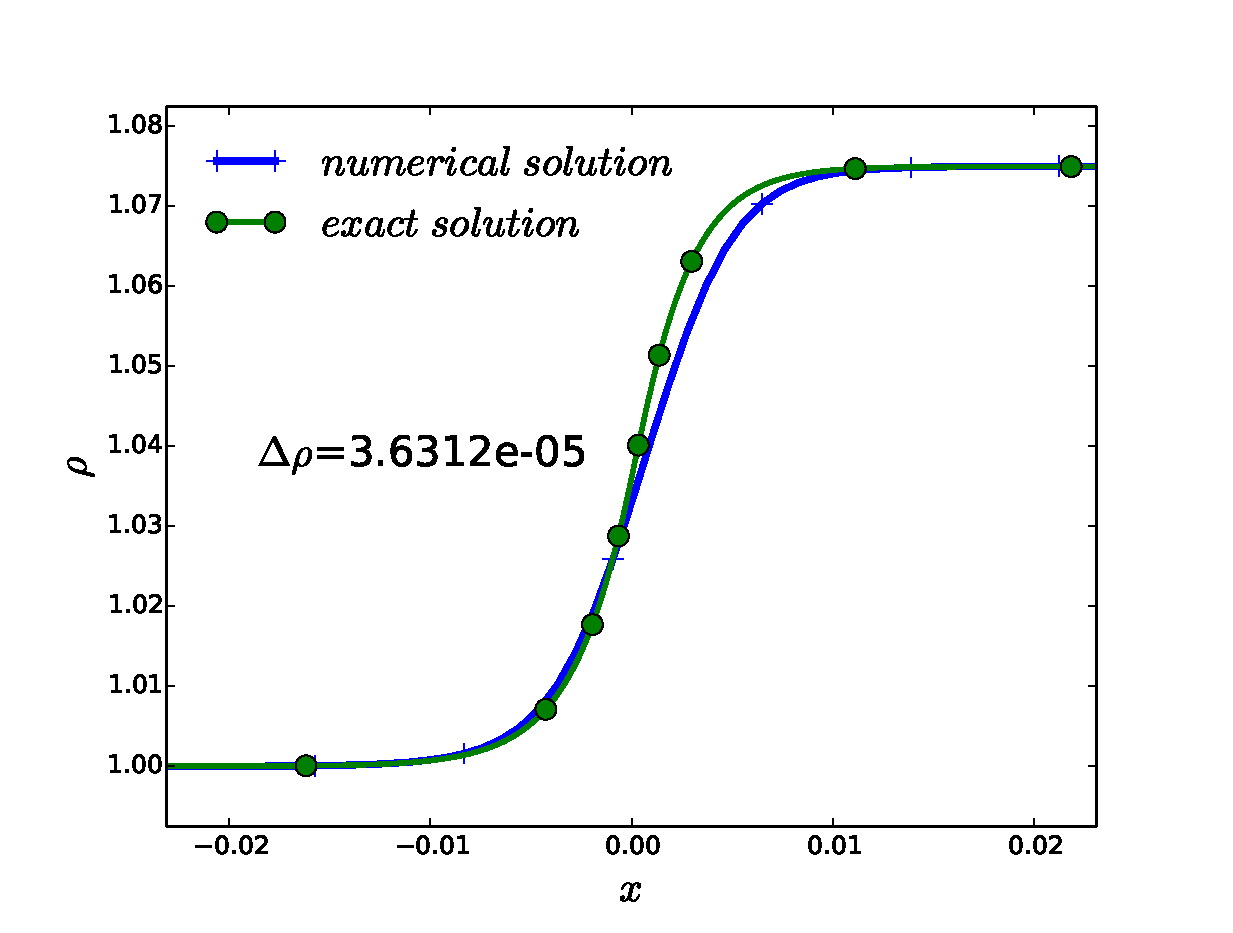
\includegraphics[width=\linewidth]{figures/cst-xs/mach-1p05/mach-1p05-density-nel-50-zero-shift.eps}
    \caption{}\label{fig:mach-1p05-cst-xs-density-no-shift}
    \end{subfigure}
    %
    \begin{subfigure}{0.49\textwidth}
    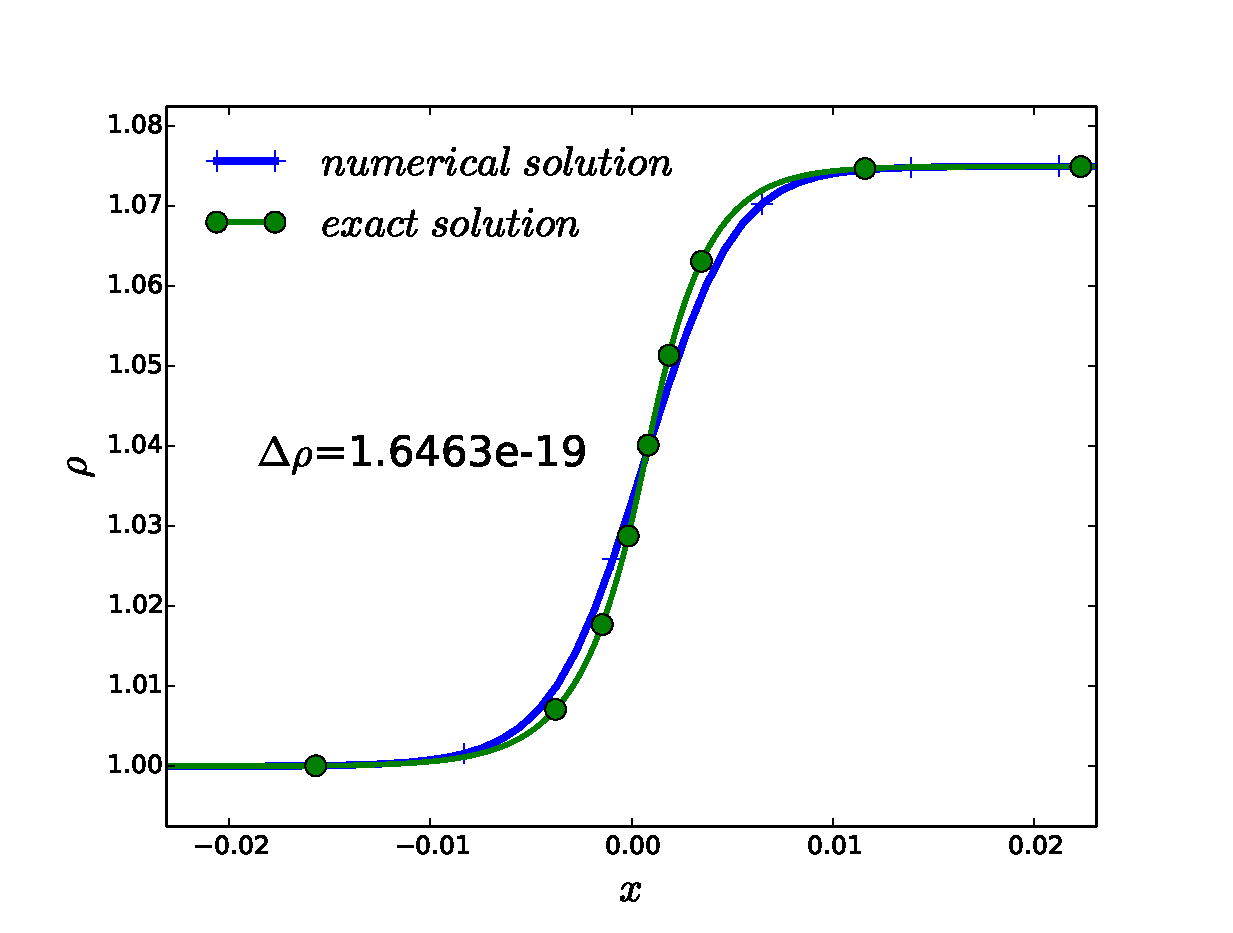
\includegraphics[width=\linewidth]{figures/cst-xs/mach-1p05/mach-1p05-density-nel-50-plot.eps}
    \caption{}\label{fig:mach-1p05-cst-xs-density-with-shift}
    \end{subfigure}
    \caption{Material density before (a) and after (b) shifting.}\label{fig:mach-1p05-shift-vs-non-shift}
\end{figure}
The convergence rates for the material density, the material temperature, the radiation temperature and the mach number are given in \fig{fig:mach-1p05-cst-xs-conv} for the $L_1$ and $L_2$ error norms.  
A reference line of slope $2$ is also provided. We observe that second-order accuracy is achieved in both the $L_1$ and $L_2$ error norms.
This example proves that the EVM achieves second-order accuracy for smooth solutions.
%
\begin{figure}[h]
    \begin{subfigure}{0.5\textwidth}
    \centering
    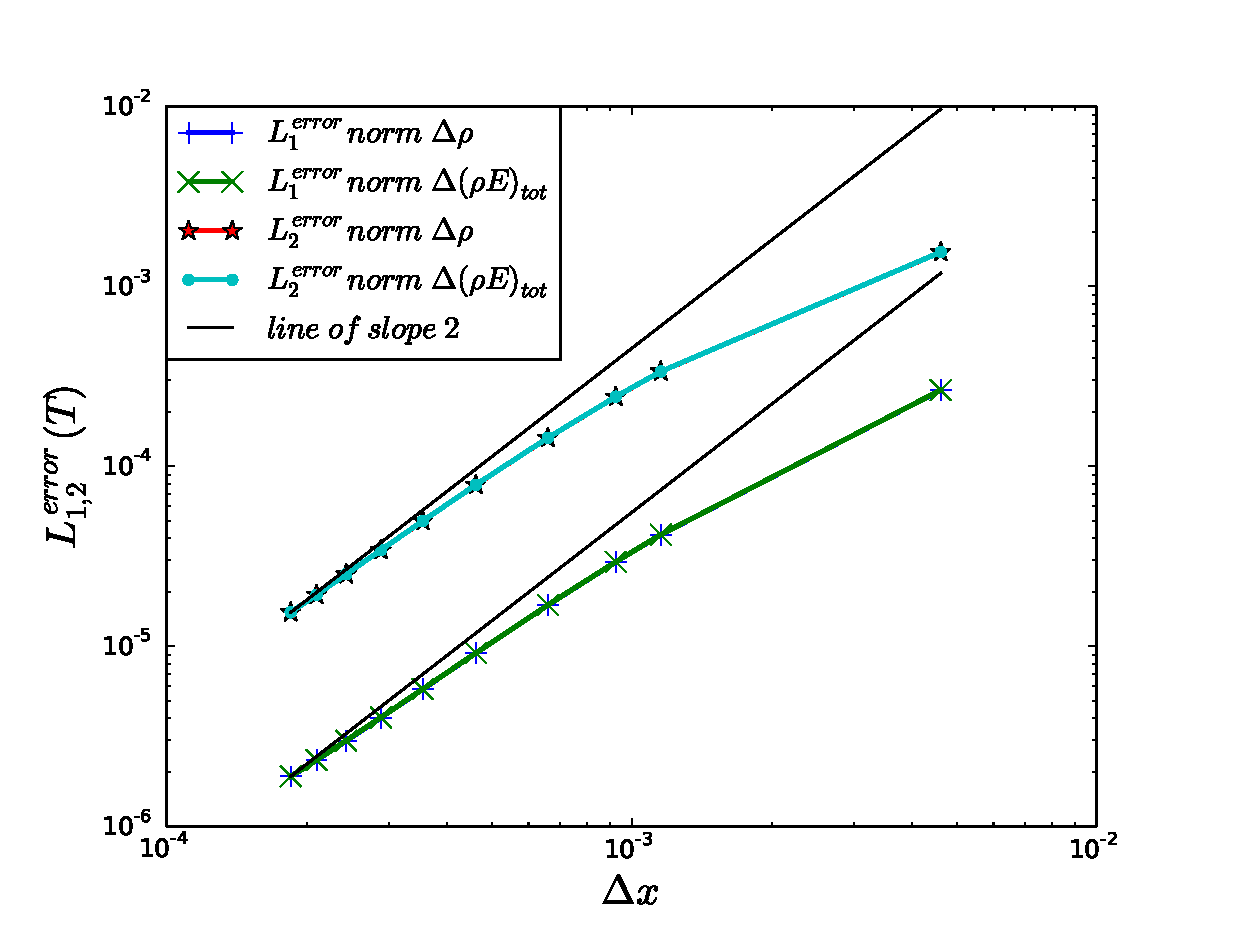
\includegraphics[width=\linewidth]{figures/cst-xs/mach-1p05/mass-energy-diff-mat-temp-convergence.eps}
    \caption{Material temperature.}\label{fig:mach-1p05-cst-xs-temp-conv}
    \end{subfigure}
    ~
    \begin{subfigure}{0.5\textwidth}
    \centering
    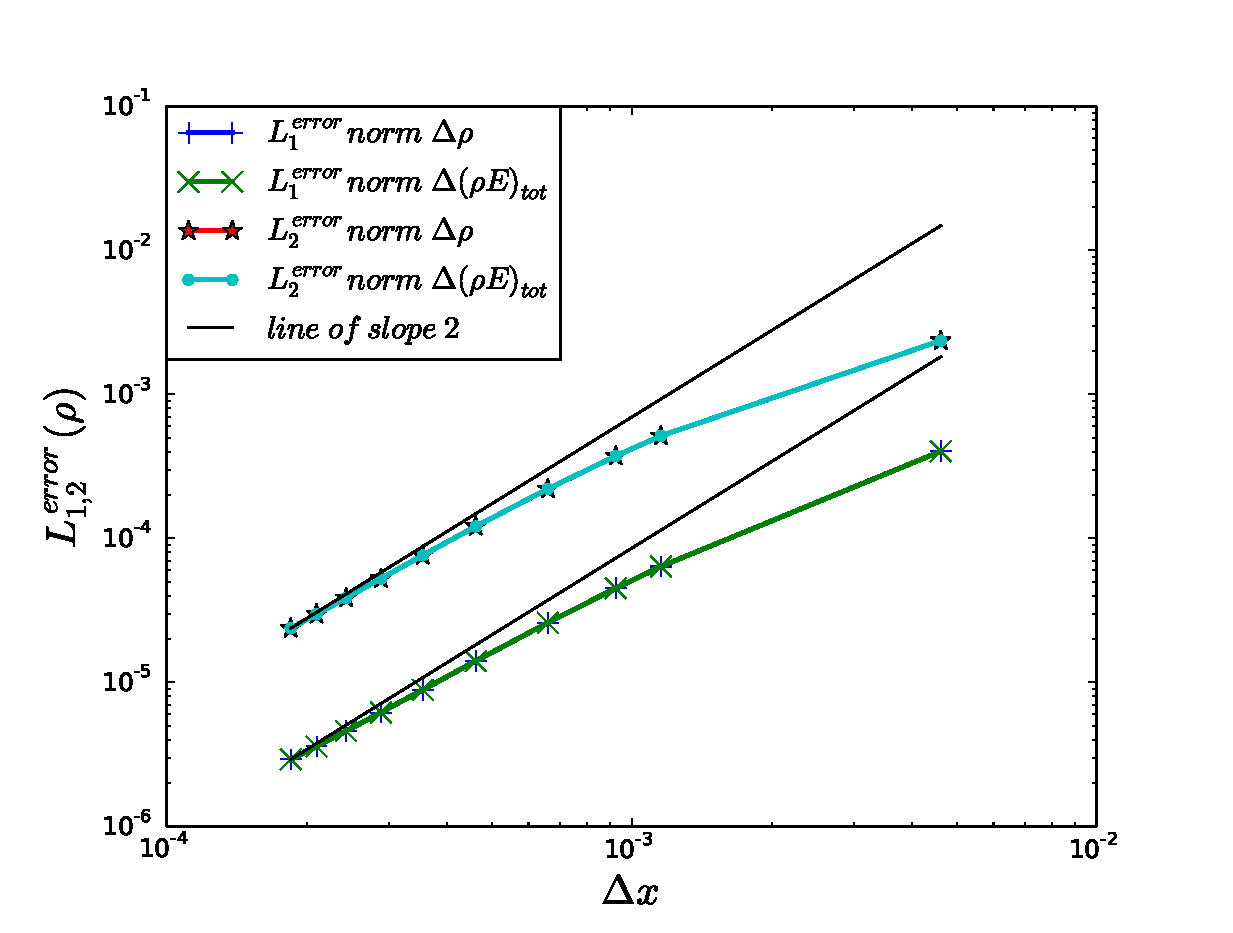
\includegraphics[width=\linewidth]{figures/cst-xs/mach-1p05/mass-energy-diff-density-convergence.eps}
    \caption{Material density.}\label{fig:mach-1p05-cst-xs-density-conv}
    \end{subfigure}
    
    \begin{subfigure}{0.5\textwidth}
    \centering
    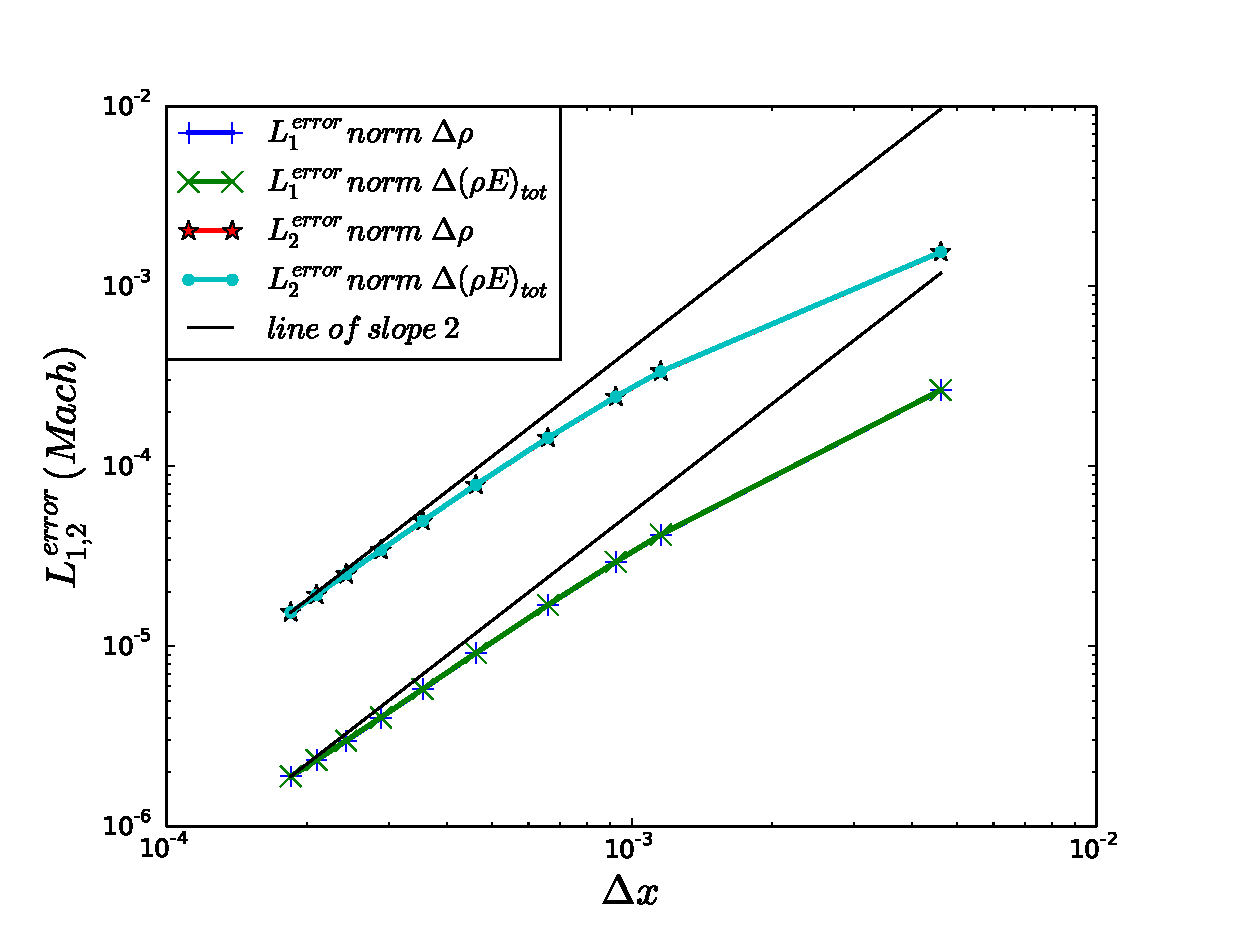
\includegraphics[width=\linewidth]{figures/cst-xs/mach-1p05/mass-energy-diff-mach-number-convergence.eps}
    \caption{Mach number.}\label{fig:mach-1p05-cst-xs-mach-conv}
    \end{subfigure}
    ~
    \begin{subfigure}{0.5\textwidth}
    \centering
    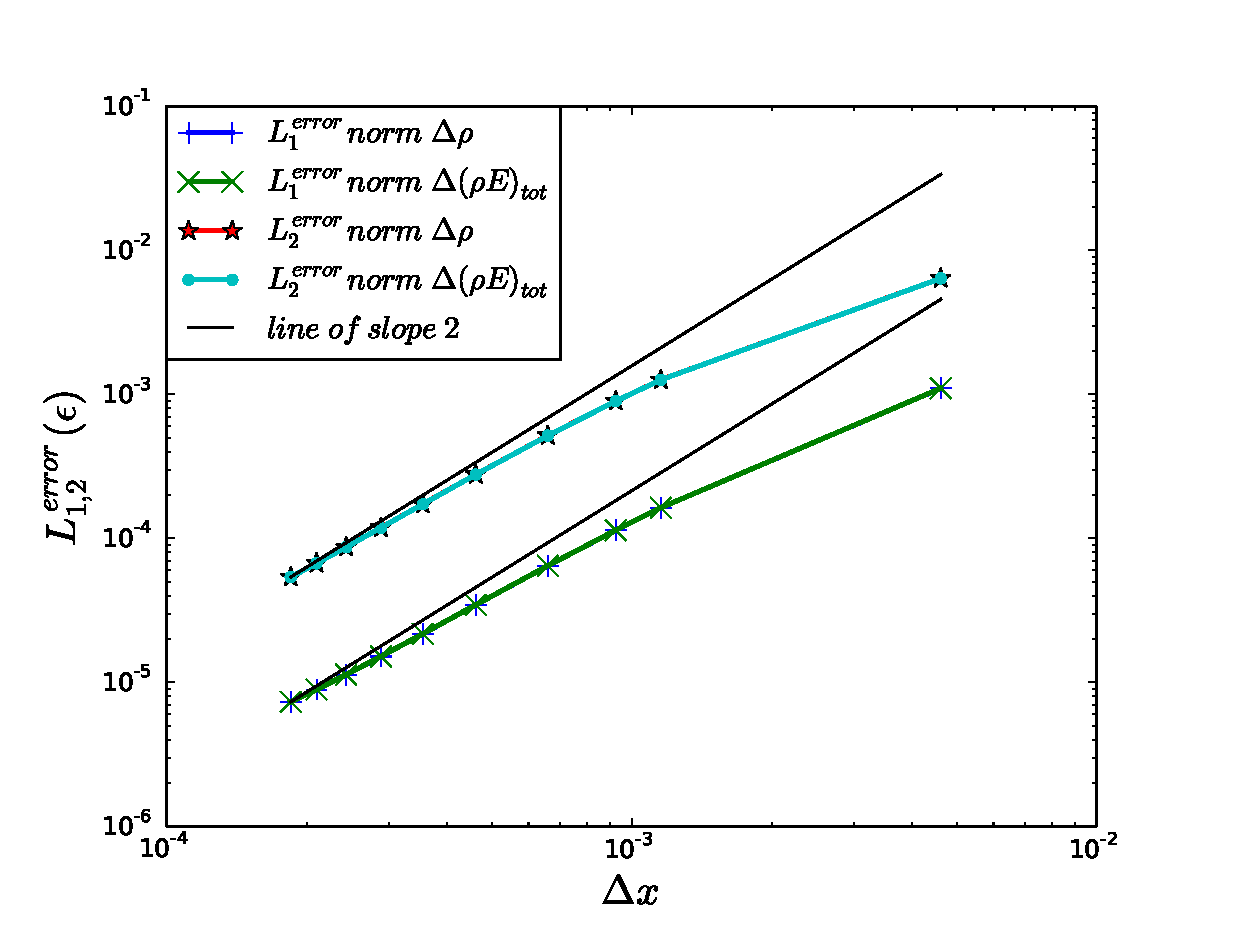
\includegraphics[width=\linewidth]{figures/cst-xs/mach-1p05/mass-energy-diff-radiation-convergence.eps}
    \caption{Radiation energy density.}\label{fig:mach-1p05-cst-xs-radiation-conv}
    \end{subfigure}        
\caption{Mach $1.05$ test: $L_1$ and $L_2$ error norms.}\label{fig:mach-1p05-cst-xs-conv}    
\end{figure}
%

The numerical and semi-analytical solutions of $(\rho, T, \epsilon, Mach)$ are plotted in \fig{fig:mach-1p05-cst-xs-density}, \fig{fig:mach-1p05-cst-xs-temp}, \fig{fig:mach-1p05-cst-xs-radiation} and \fig{fig:mach-1p05-cst-xs-mach}, respectively. We note that the numerical solution is smooth and in excellent agreement with the semi-analytical solution for each variable. The viscosity coefficients $\kappa$ and $\kappa_\text{max}$ are plotted in \fig{fig:mach-1p05-cst-xs-visc} on a log-scale. The entropy viscosity coefficient $\kappa$ is three to seven orders of magnitude smaller than the first-order viscosity coefficient $\kappa_\text{max}$. Such behavior is expected as the numerical solution is smooth and the entropy production small.
%
\begin{figure}[h]
    \centering
    \begin{subfigure}{0.49\textwidth}
    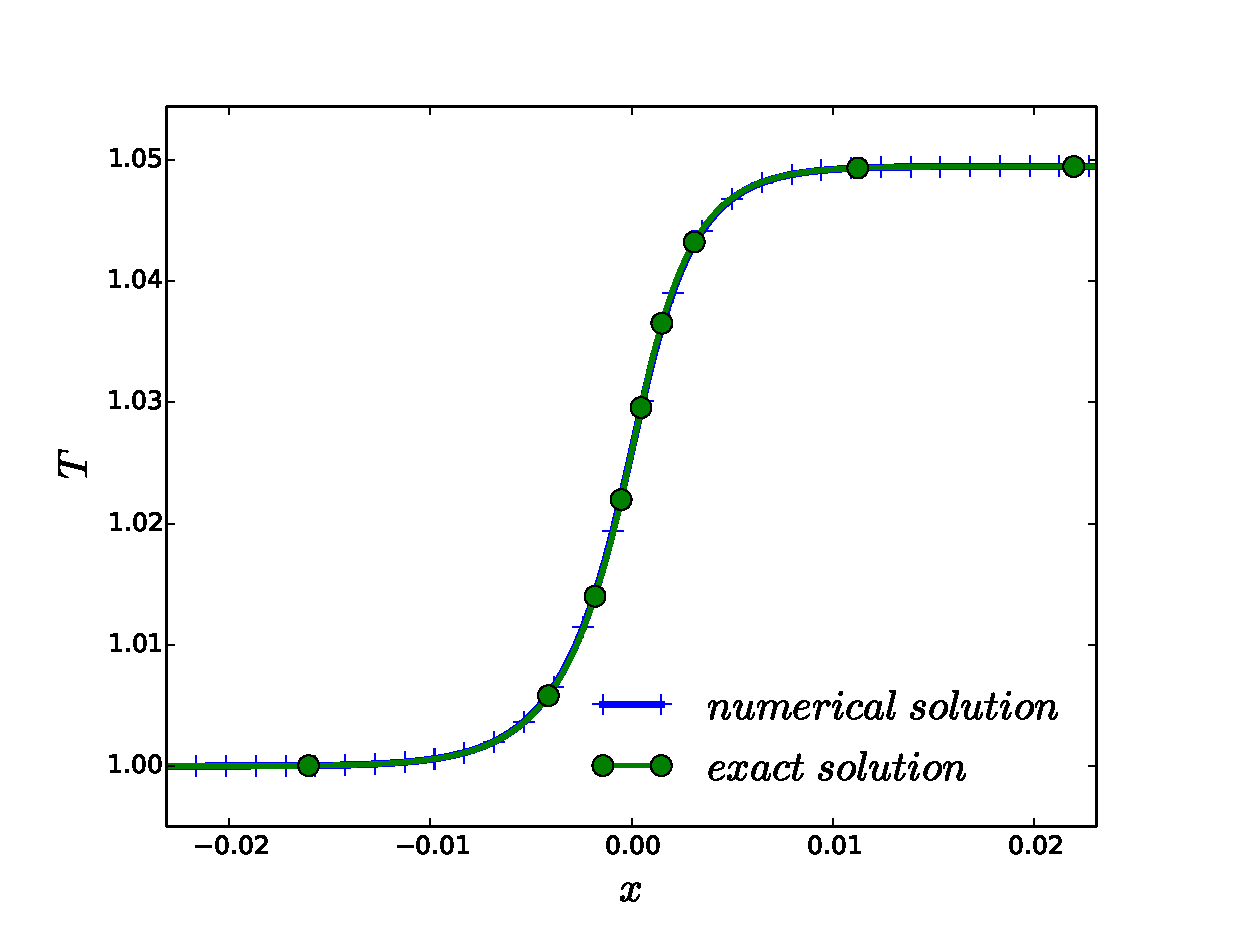
\includegraphics[width=\linewidth]{figures/cst-xs/mach-1p05/mass-diff-mach-1p05-mat-temp-nel-250-plot.eps}
    \caption{Material temperature.}\label{fig:mach-1p05-cst-xs-temp}
    \end{subfigure}
    \begin{subfigure}{0.49\textwidth}
    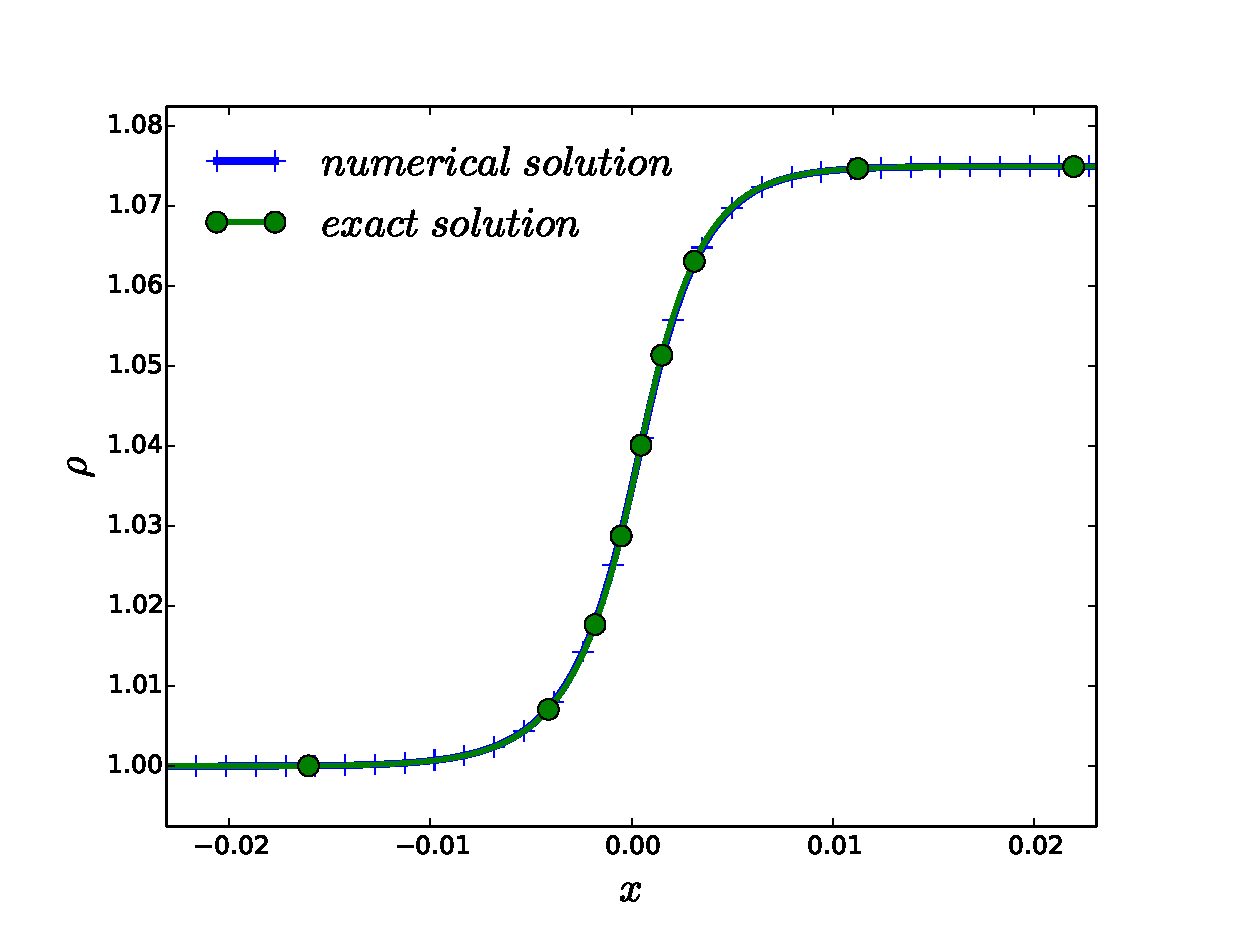
\includegraphics[width=\linewidth]{figures/cst-xs/mach-1p05/mass-diff-mach-1p05-density-nel-250-plot.eps}
    \caption{Material density.}\label{fig:mach-1p05-cst-xs-density}
    \end{subfigure}
    \begin{subfigure}{0.49\textwidth}
    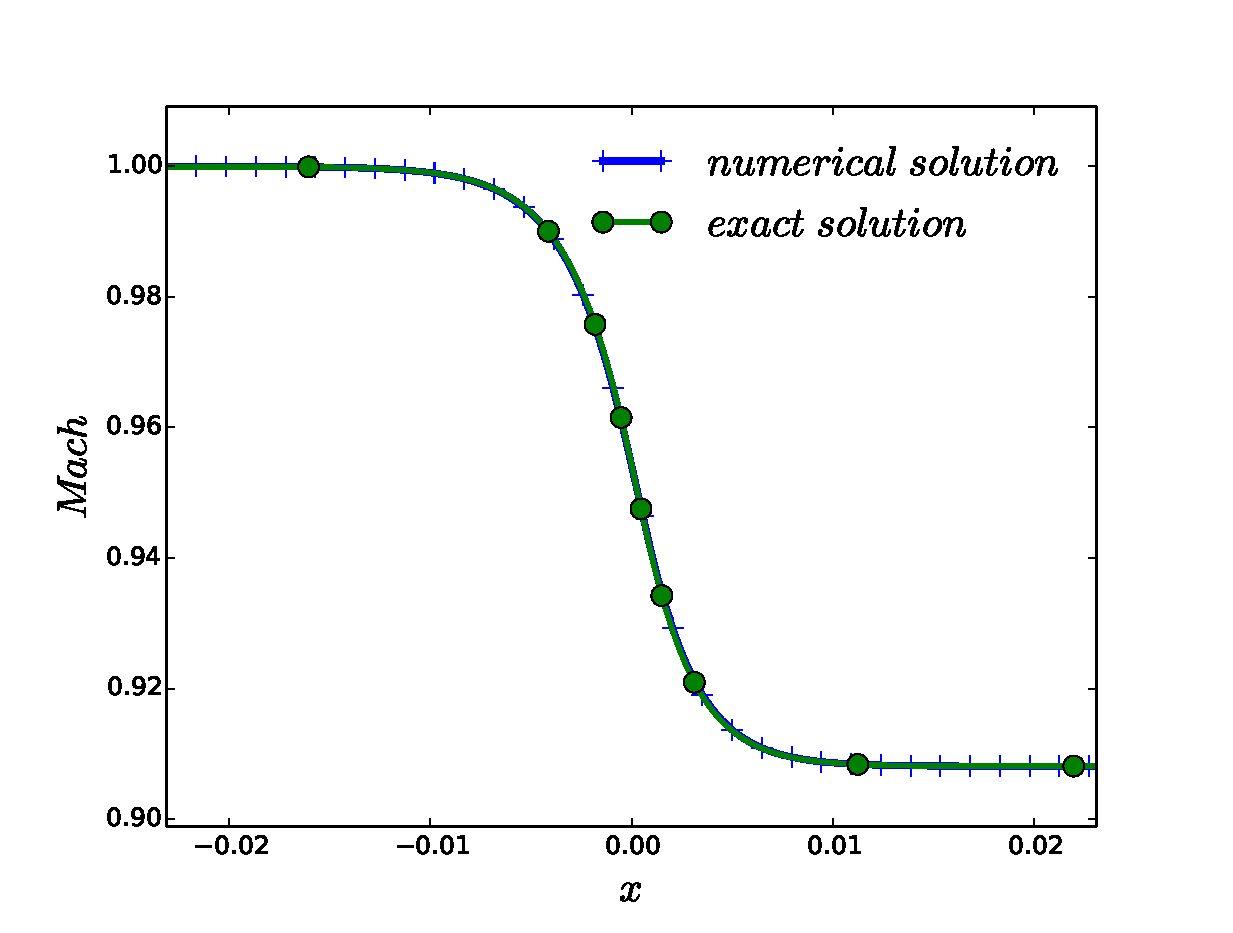
\includegraphics[width=\linewidth]{figures/cst-xs/mach-1p05/mass-diff-mach-1p05-mach-number-nel-250-plot.eps}
    \caption{Mach number.}\label{fig:mach-1p05-cst-xs-mach}
    \end{subfigure}
    \begin{subfigure}{0.49\textwidth}
    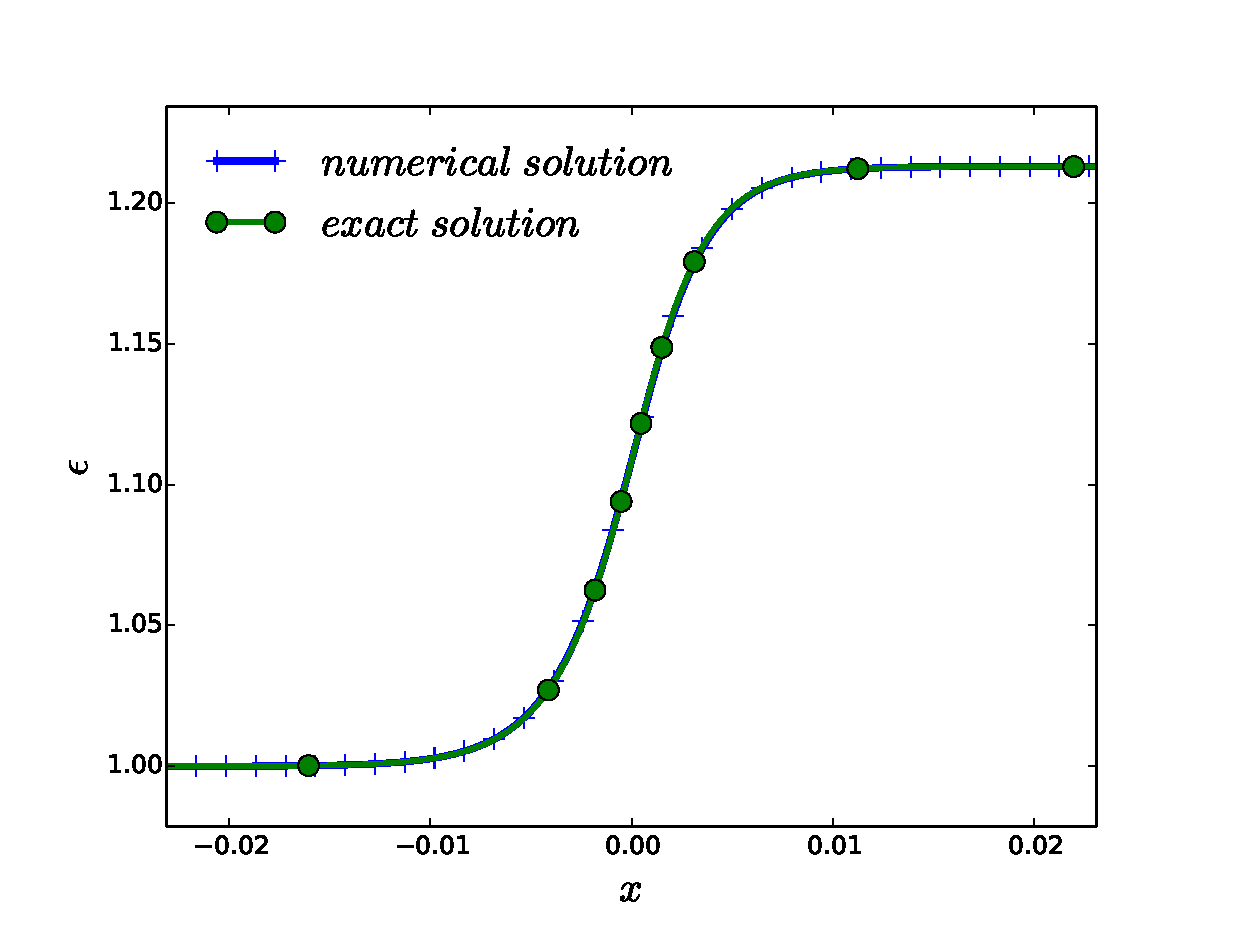
\includegraphics[width=\linewidth]{figures/cst-xs/mach-1p05/mass-diff-mach-1p05-radiation-nel-250-plot.eps}
    \caption{Radiation energy density.}\label{fig:mach-1p05-cst-xs-radiation}
    \end{subfigure}        
    \begin{subfigure}{0.49\textwidth}
    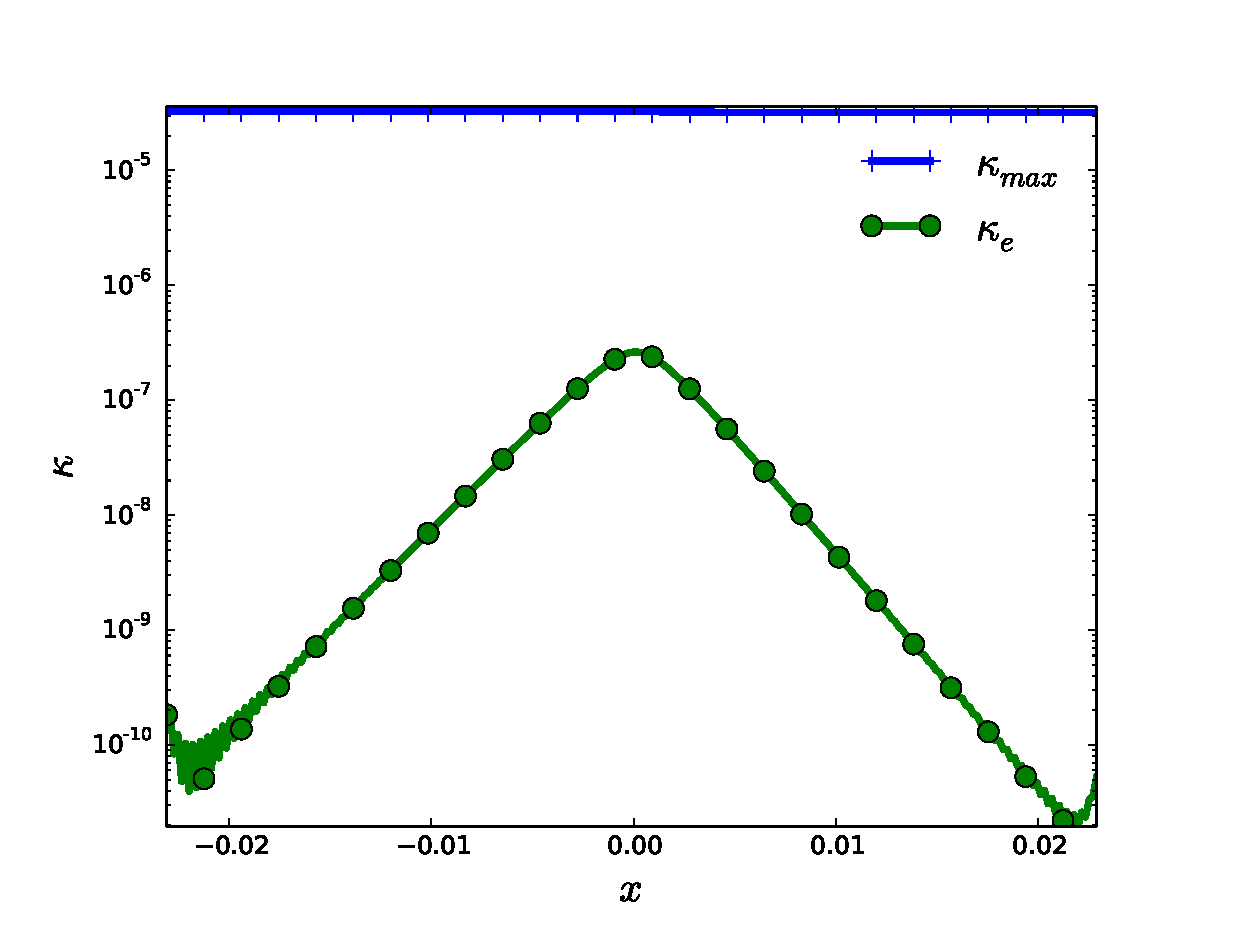
\includegraphics[width=\linewidth]{figures/cst-xs/mach-1p05/mass-diff-mach-1p05-visc-nel-250-plot.eps}
    \caption{Viscosity coefficients.}\label{fig:mach-1p05-cst-xs-visc}
    \end{subfigure}        
\caption{Mach $1.05$ test with constant opacity: Numerical ($250$ cells) and semi-analytical ($\sim 3500$ nodes) steady-state profiles;
material temperature (a), density (b), radiation energy (c), Mach number (d), and viscosity coefficient coefficient (e).}\label{fig:mach-1p05-cst-xs}    
\end{figure}
\FloatBarrier
\newpage
\pagebreak
\newpage

%------------------------------------------------------------------
\subsection{Mach-3 shock test with constant opacity}\label{sec:mach-3-cst-xs}
%------------------------------------------------------------------
%
In this test case, the inlet Mach number is set to $3$ and the total and absorption opacities are still assumed constant. 
The purpose of this test is twofold: (i) it shows that the EVM achieves first-order accuracy for numerical solutions with shocks, and, (ii) it illustrates the point made in \sct{sec:VR_new}, i.e., that the source terms positively contribute to the stabilization of the numerical solution.

A convergence study is performed for the variables $(\rho, T, \epsilon, Mach)$ by following the method given previous in \sct{sec:mthd-conv-test} on successively refined grids with spatial mesh sizes ranging from $\sim 10^{-5}$ to $\sim 10^{-3}$ $cm$. The $L_1$ error norms computed with mass ($\Delta \rho$) and energy ($\Delta (\rho E)_{tot}$) conversation procedures are given in \fig{fig:mach-3-cst-xs-conv}; the semi-analytical solution used $5 \times 10^4$ nodes. A reference line of slope 1 shows that first-order convergence in the $L_1$ error is achieved for either conservation procedures. A convergence rate of 1 is expected for a numerical solution developing a shock \cite{lowrie-2009} 
(note that only convergence plots for the material temperature are provided in \cite{lowrie-2009}). 
We also note that in the pre-asymptotic range, the radiation energy variable exhibits second-order convergence, before leveling off
to a first-order convergence rate, see \fig{fig:mach-3-cst-xs-radiation-conv}.  
Given that the radiation energy variable is always smooth, even in the shock region, a higher convergence rate is possible
until the first-order rate present in the other (hydrodynamic) variables limits the radiation energy rate to unity.
This behavior may warrant further analysis. 
%
\begin{figure}[ht]
    \begin{subfigure}{0.5\textwidth}
    \centering
    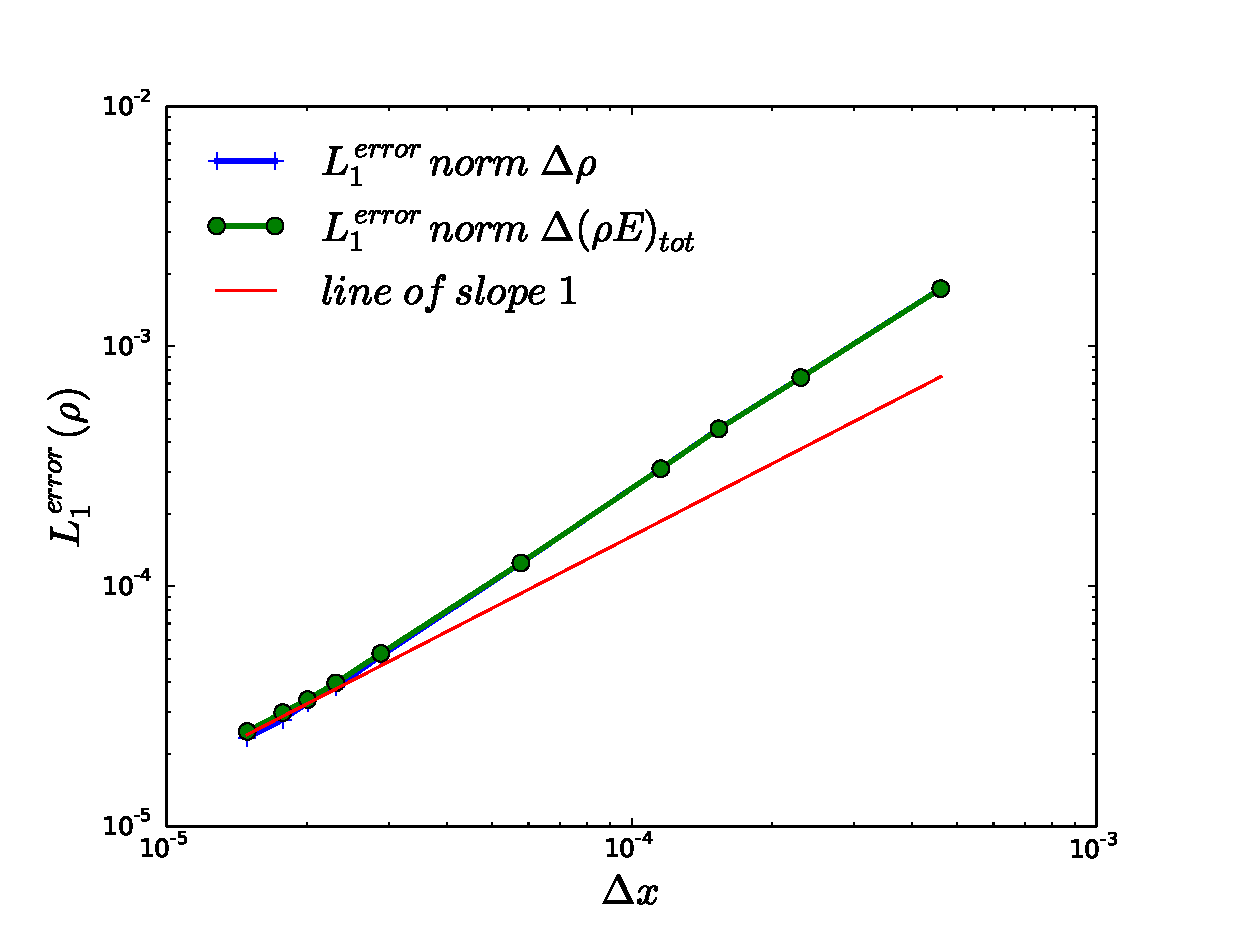
\includegraphics[width=\linewidth]{figures/cst-xs/mach-3/mass-energy-diff-scd-method-density-convergence.eps}
    \caption{Material density.}\label{fig:mach-3-cst-xs-density-conv}
    \end{subfigure}
    ~
    \begin{subfigure}{0.5\textwidth}
    \centering
    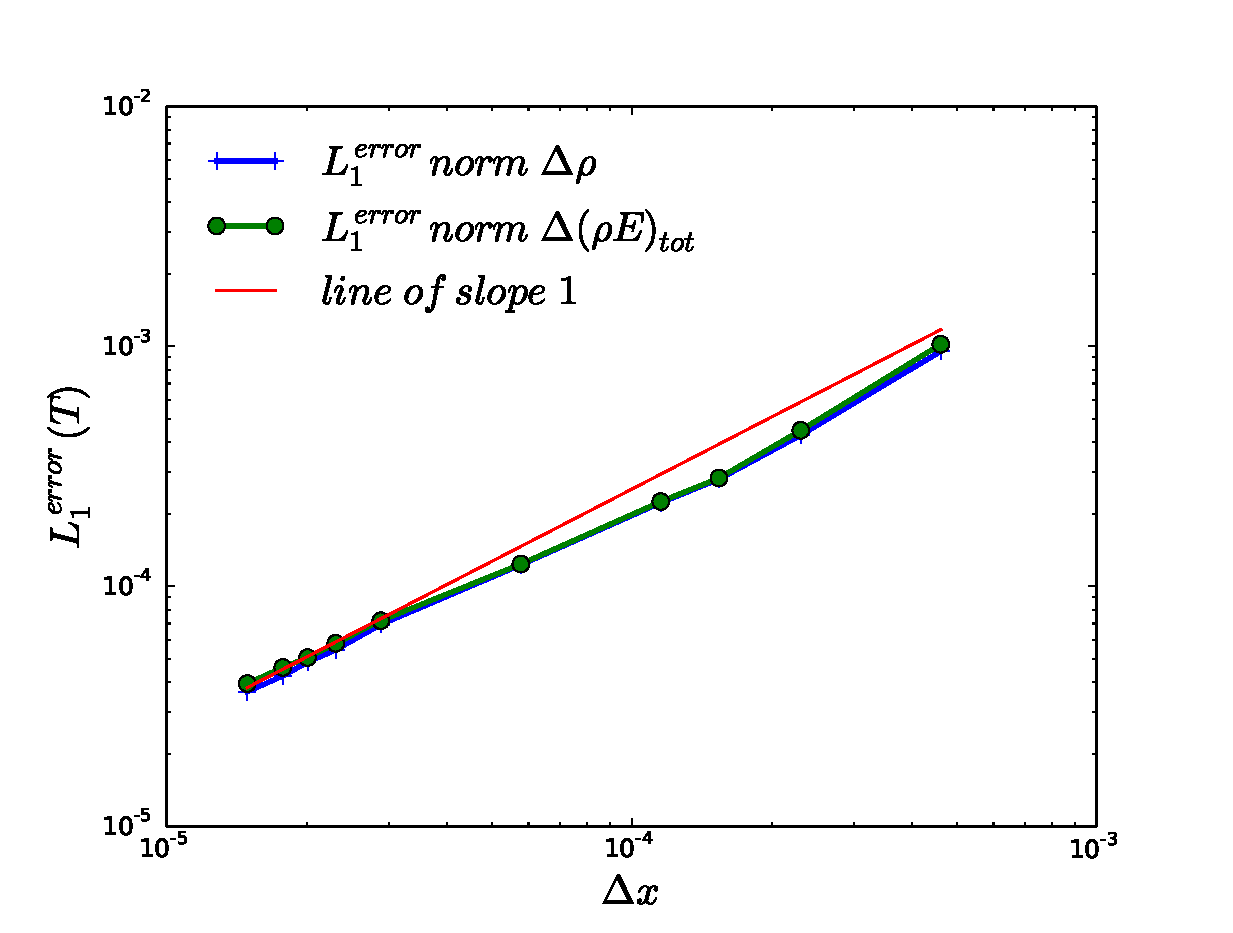
\includegraphics[width=\linewidth]{figures/cst-xs/mach-3/mass-energy-diff-scd-method-mat-temp-convergence.eps}
    \caption{Material temperature.}\label{fig:mach-3-cst-xs-temp-conv}
    \end{subfigure}
    
    \begin{subfigure}{0.5\textwidth}
    \centering
    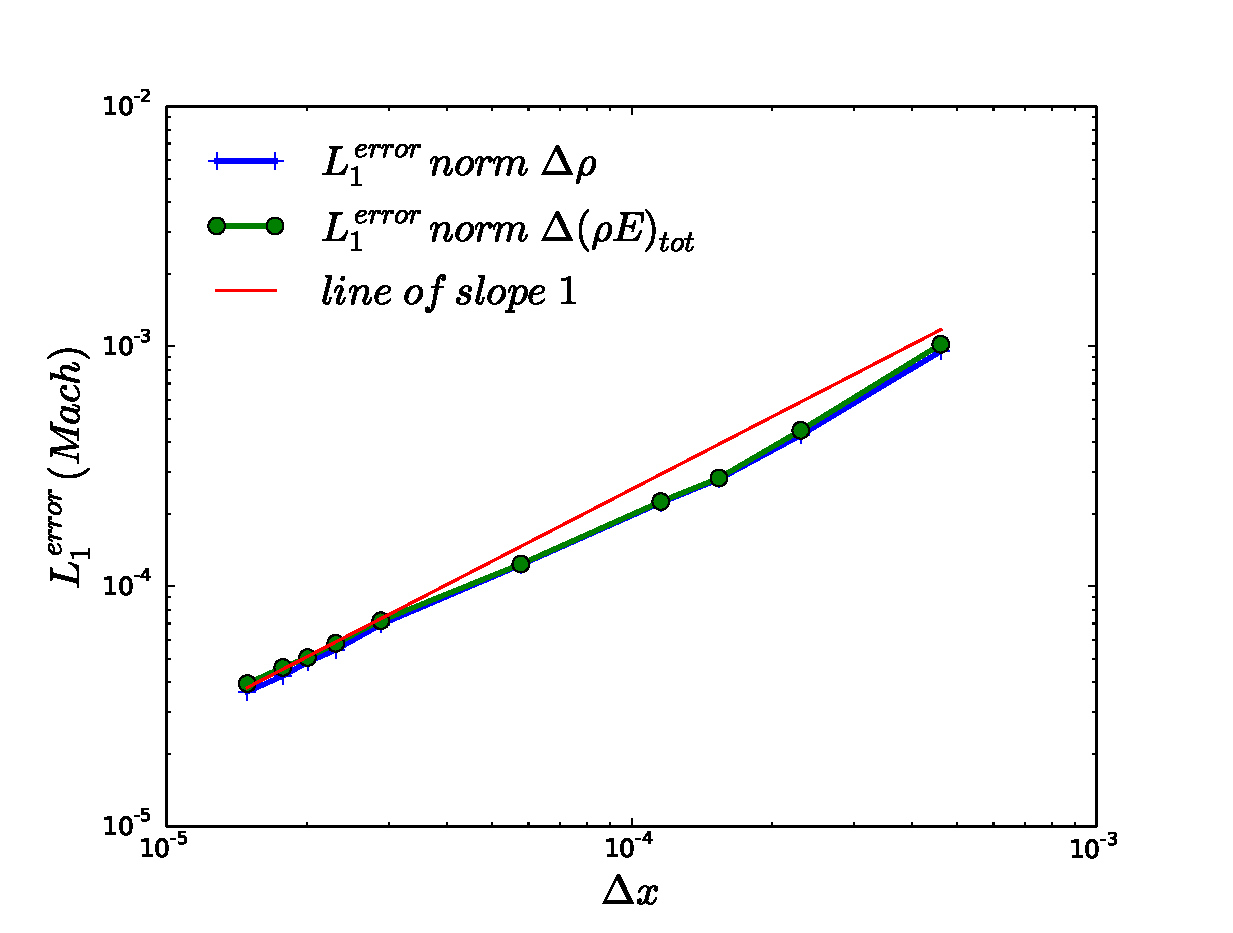
\includegraphics[width=\linewidth]{figures/cst-xs/mach-3/mass-energy-diff-scd-method-mach-number-convergence.eps}
    \caption{Mach number.}\label{fig:mach-3-cst-xs-mach-conv}
    \end{subfigure}
    ~
    \begin{subfigure}{0.5\textwidth}
    \centering
    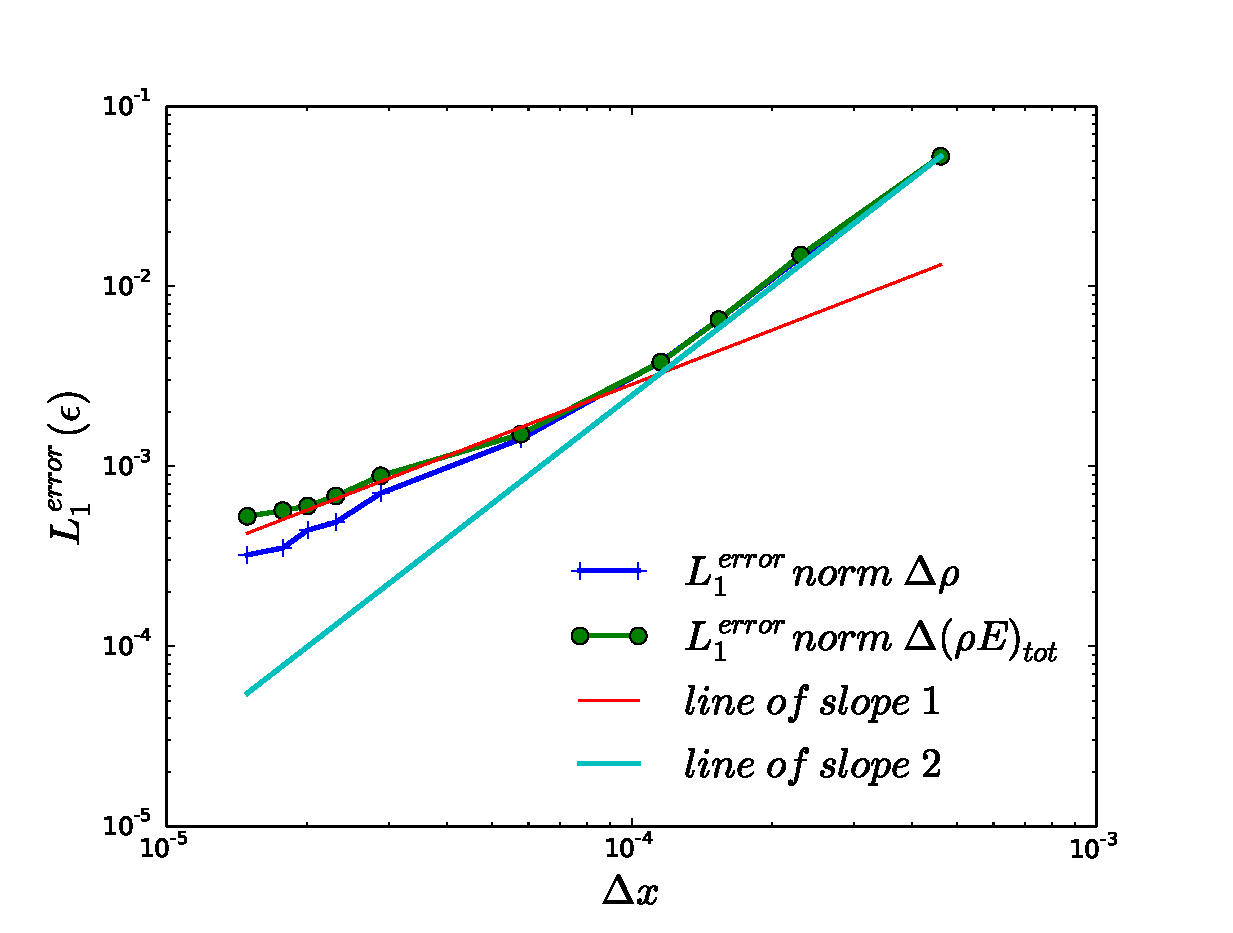
\includegraphics[width=\linewidth]{figures/cst-xs/mach-3/mass-energy-diff-scd-method-radiation-convergence.eps}
    \caption{Radiation energy density.}\label{fig:mach-3-cst-xs-radiation-conv}
    \end{subfigure}        
\caption{Mach $3$ test with constant opacity: $L_1$ error norms}\label{fig:mach-3-cst-xs-conv}    
\end{figure}
%

The numerical solution obtained with a spatial mesh size of $\Delta x \sim 10^{-4}$ $cm$ are plotted against the semi-analytical solutions 
along with the viscosity coefficients $\kappa$ and $\kappa_\text{max}$ in \fig{fig:mach-3-cst-xs}. All variables show good agreement with the semi-analytical solution. A shock is located around $x=0$ in the material density and Mach number profiles in \fig{fig:mach-3-cst-xs-dens} and \fig{fig:mach-3-cst-xs-mach}, respectively. The shock is well resolved and the numerical solution does not display any instabilities (over/undershoots). In \fig{fig:mach-3-cst-xs-temp}, the material temperature profile displays a Zeldovich's spike in the vicinity of the shock region: the spike is well resolved and matches the semi-analytical solution. On the other hand, the radiation energy density shown in \fig{fig:mach-3-cst-xs-rad} remains smooth even in the vicinity of the peak because of the diffusion term $ \partial_x \left( \frac{c}{3 \sigma_t} \partial_x \epsilon \right)$ in the radiation equation (\eqt{eq:GRHrad}). The viscosity coefficients $\kappa$ and $\kappa_\text{max}$ are plotted in \fig{fig:mach-3-cst-xs-visc} on a log-scale. We observe that $\kappa$ is peaked in the vicinity of the shock and small elsewhere. This behavior is in agreement with the underlying principles invoked in the definition of the viscosity coefficient $\kappa$, that is, $\kappa$
should be proportional to the local entropy residual. We also note that the viscosity coefficient $\kappa$ does not saturate to the first-order viscosity coefficient $\kappa_\text{max}$ but still efficiently stabilizes the numerical solution. This is a consequence of the point explained in \sct{sec:VR_new} that highlights the entropy-producing effects, i.e., stabilizing effects, of the relaxation and the diffusion terms (see \eqt{eq:ineq_ent_eq}).
%
\begin{figure}[h]
    \centering
    \begin{subfigure}{0.49\textwidth}
    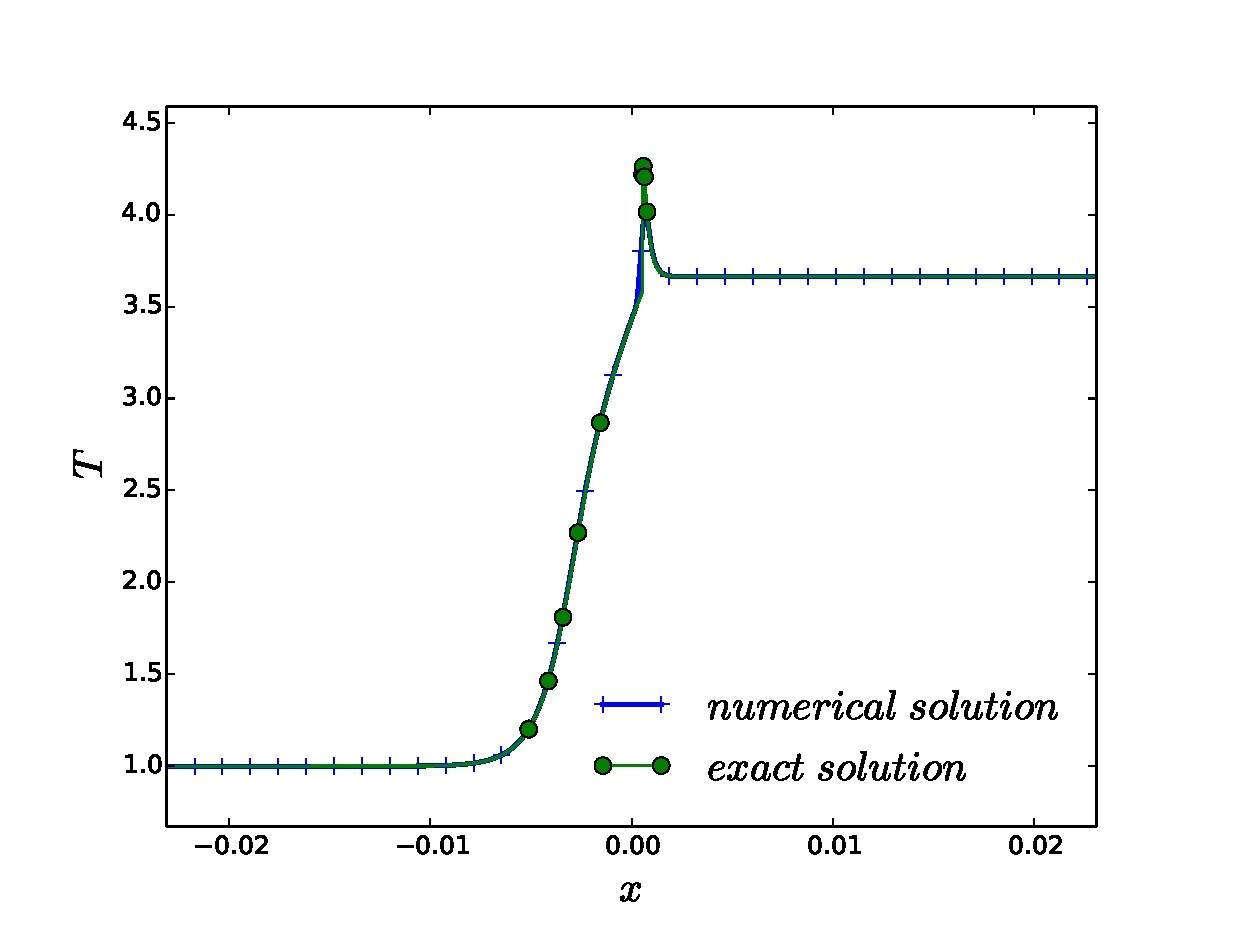
\includegraphics[width=\linewidth]{figures/cst-xs/mach-3/mass-diff-mat-temp-nel-1000-plot.eps}
    \caption{Material temperature.}\label{fig:mach-3-cst-xs-temp}
    \end{subfigure}	
%
    \begin{subfigure}{0.49\textwidth}
    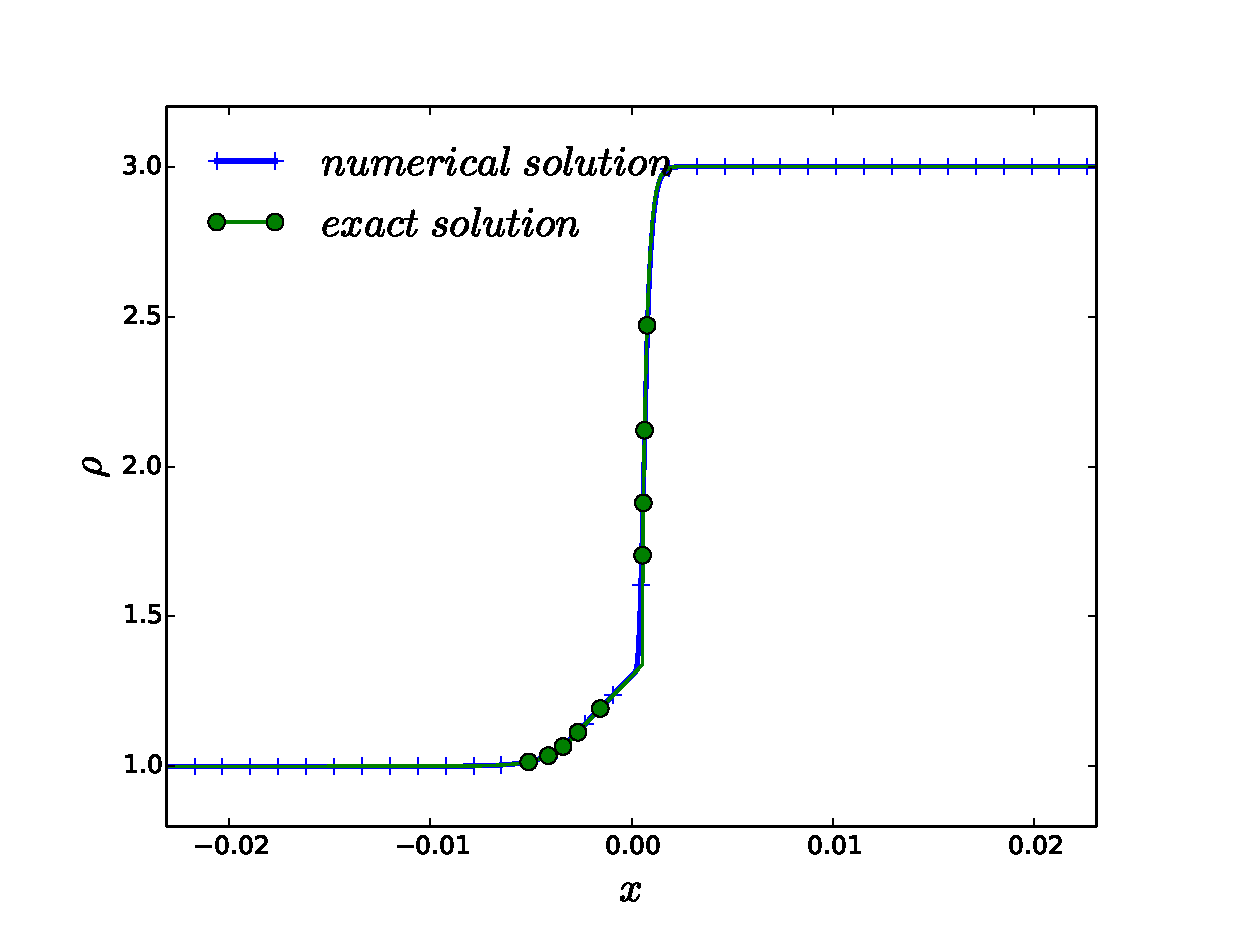
\includegraphics[width=\linewidth]{figures/cst-xs/mach-3/mass-diff-density-nel-1000-plot.eps}
    \caption{Material density.}\label{fig:mach-3-cst-xs-dens}
    \end{subfigure}
%
    \begin{subfigure}{0.49\textwidth}
    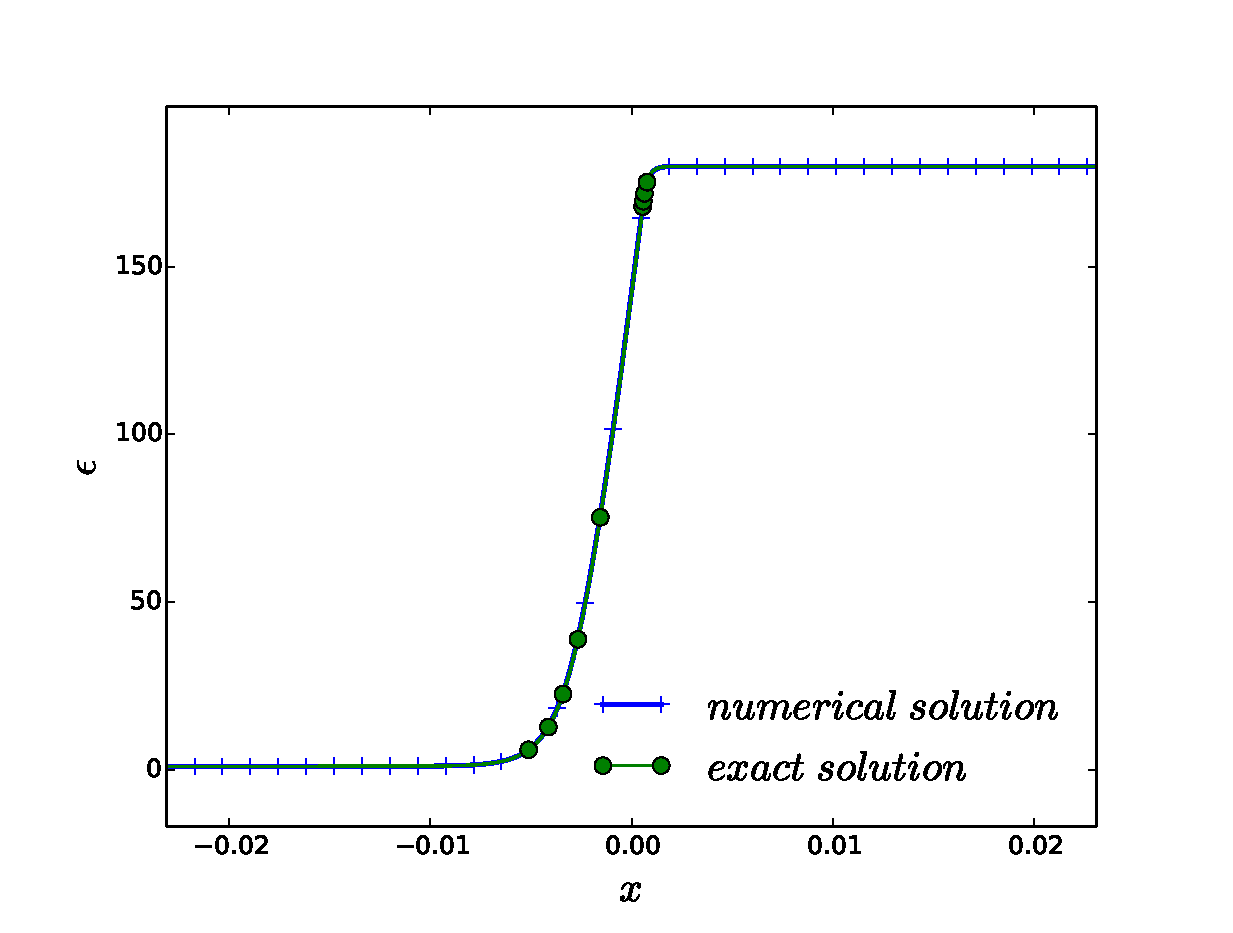
\includegraphics[width=\linewidth]{figures/cst-xs/mach-3/mass-diff-radiation-nel-1000-plot.eps}
    \caption{Radiation energy density.}\label{fig:mach-3-cst-xs-rad}
    \end{subfigure}
%   
    \begin{subfigure}{0.49\textwidth}
    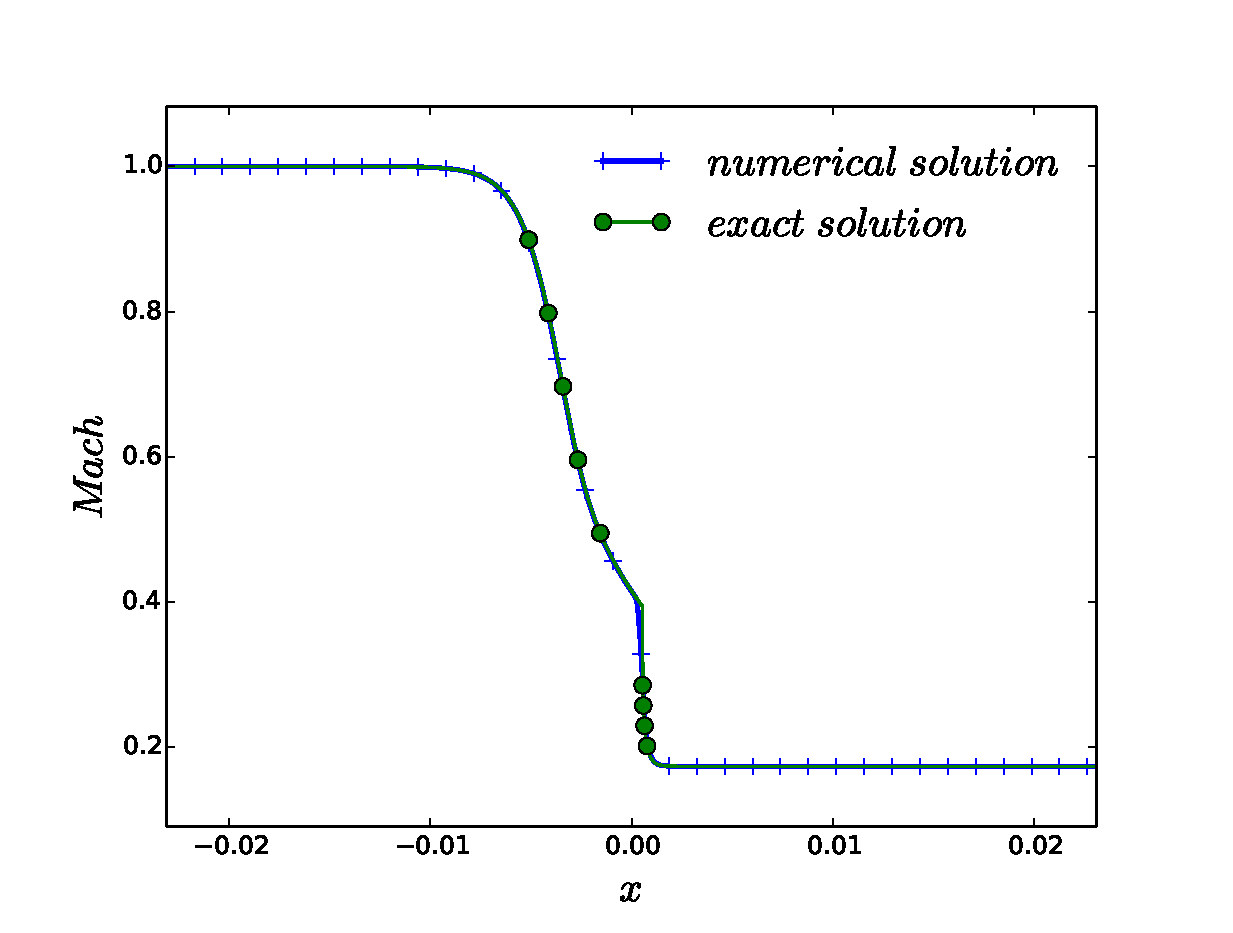
\includegraphics[width=\linewidth]{figures/cst-xs/mach-3/mass-diff-mach-number-nel-1000-plot.eps}
    \caption{Mach number.}\label{fig:mach-3-cst-xs-mach}
    \end{subfigure}
%
    \begin{subfigure}{0.49\textwidth}
    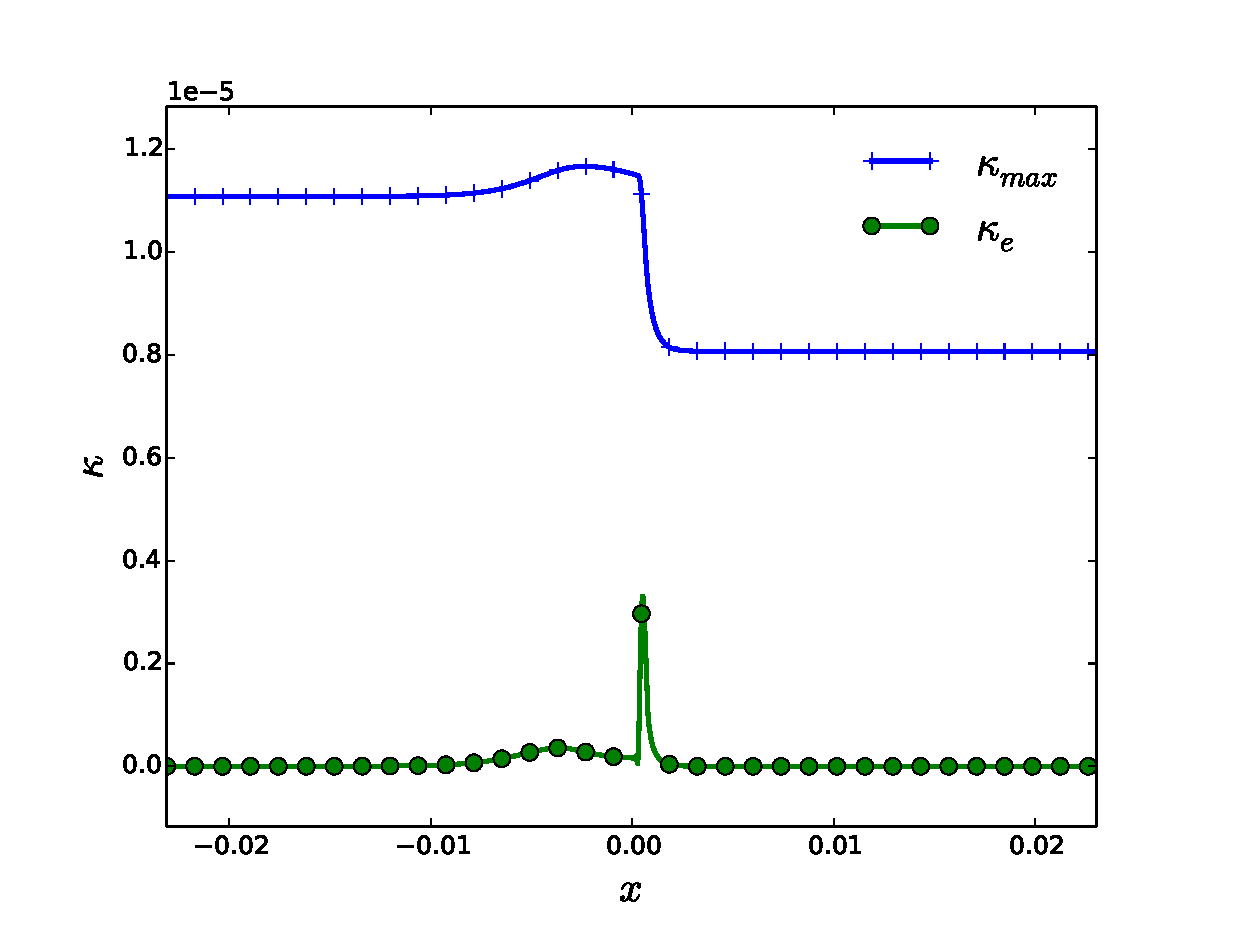
\includegraphics[width=\linewidth]{figures/cst-xs/mach-3/mass-diff-visc-nel-1000-plot.eps}
    \caption{Artificial viscosity coefficients.}\label{fig:mach-3-cst-xs-visc}
    \end{subfigure}        
\caption{Mach $3$ test with constant opacity: Numerical ($1000$ cells) and semi-analytical ($\sim 5 \cdot 10^4$ nodes) steady-state profiles for the material temperature (a),  density (b),  radiation temperature (c), Mach number (d), and  viscosity coefficient (e).}\label{fig:mach-3-cst-xs}      
\end{figure}
%

%------------------------------------------------------------------
\subsection{Mach-3 shock test with temperature- and density-dependent opacity}\label{sec:mach-3-no-cst-xs}
%------------------------------------------------------------------
%
We now consider a Mach 3 test in a pure absorber material with the same initial conditions as in \sct{sec:mach-3-cst-xs} but with an opacity that depends on the a-dimensional material properties, i.e., density $\hat{\rho}$ and temperature $\hat{T}$. An expression of the \emph{dimensional} form of the density- and  temperature-dependent opacity is given in \eqt{eq:opacity}:
%
\begin{equation}\label{eq:opacity}
\sigma_a(\hat{\rho},\hat{T}) = \sigma_t(\hat{\rho},\hat{T}) = \hat{\rho} \frac{577.35}{\hat{T}^{3.5}} \ cm^{-1}\, .
\end{equation}
%
This simulation aims at exercising the entropy viscosity method with an opacity function that exhibits strong variations in the shock region. From a theoretical perspective, as shown in \sct{sec:VR_new}, the entropy inequality holds, meaning that the viscous regularization should efficiently stabilize any discontinuity or shock that may form in the numerical solution. 

Once again, a convergence study at steady state in the $L_1$ error norm is performed for the variables $(\rho, T, \epsilon, Mach)$ and plots are shown in \fig{fig:mach-3-dpt-xs-conv} . A reference line of slope 1 shows that first-order convergence in the $L_1$ error norm is achieved for all variables, as expected for a numerical solution containing a shock. Here again, the radiation energy density convergence rate in \fig{fig:mach-3-dpt-xs-radiation-conv} displays a higher convergence rate in pre-asymptotic region, i.e., the radiation energy density achieves second-order accuracy for $\Delta x \geq 10^{-4}$ even though the material variables are only first-order accurate. 
Numerical results for the material density, the material temperature and the radiation energy density are plotted against semi-analytical solutions in \fig{fig:mach-3-dpt-xs-dens}, \fig{fig:mach-3-dpt-xs-mat-temp} and \fig{fig:mach-3-dpt-xs-rad-temp}, respectively. We also provide plots of the viscosity coefficient in \fig{fig:mach-3-dpt-xs-visc} and the opacity in \fig{fig:mach-3-dpt-xs-xs}.
%
\begin{figure}[ht]
    \centering
    \begin{subfigure}{0.49\textwidth}
    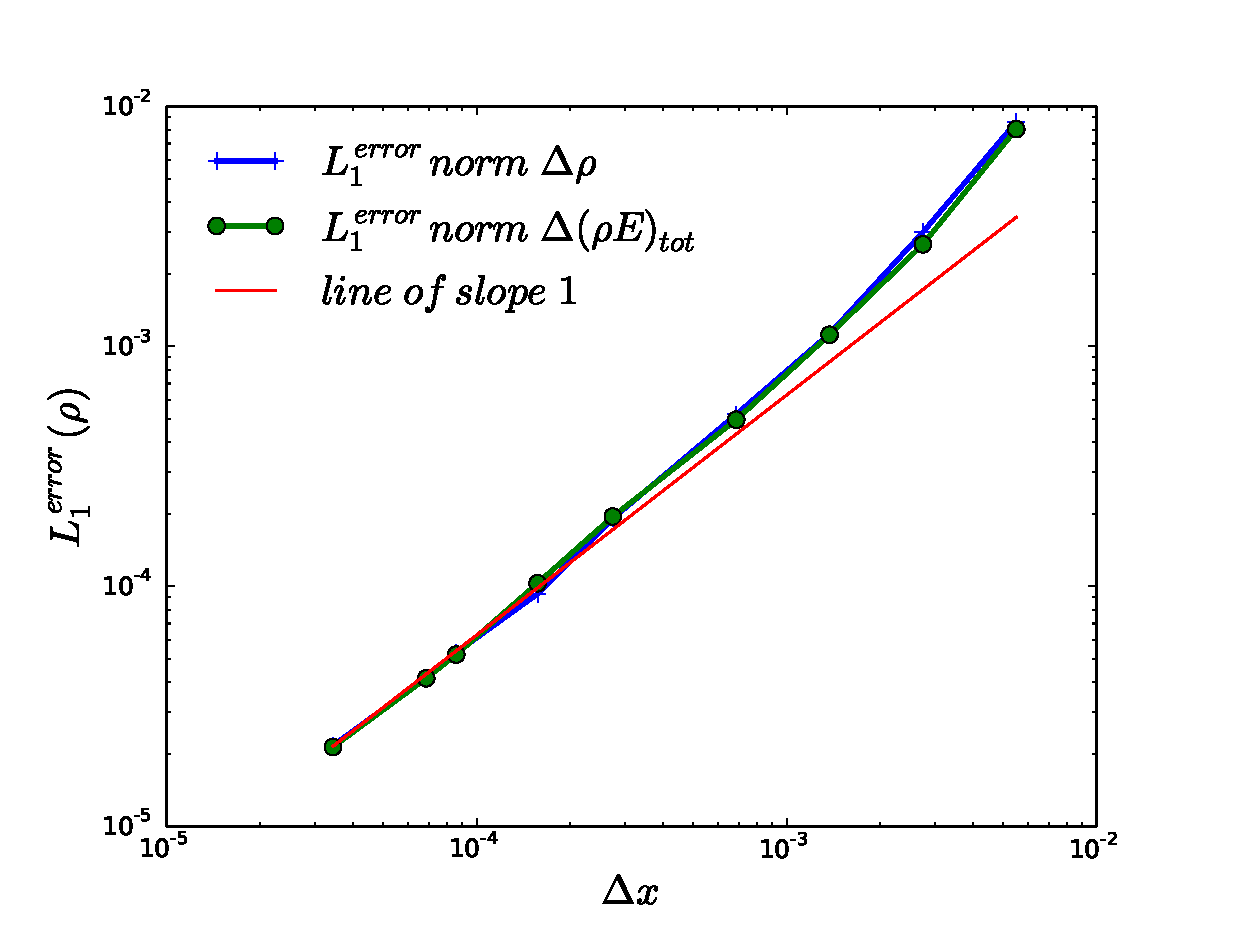
\includegraphics[width=\linewidth]{figures/dpt-xs/mass-energy-diff-scd-method-density-convergence.eps}
    \caption{Material density.}\label{fig:mach-3-dpt-xs-density-conv}
    \end{subfigure}
%
    \begin{subfigure}{0.49\textwidth}    
    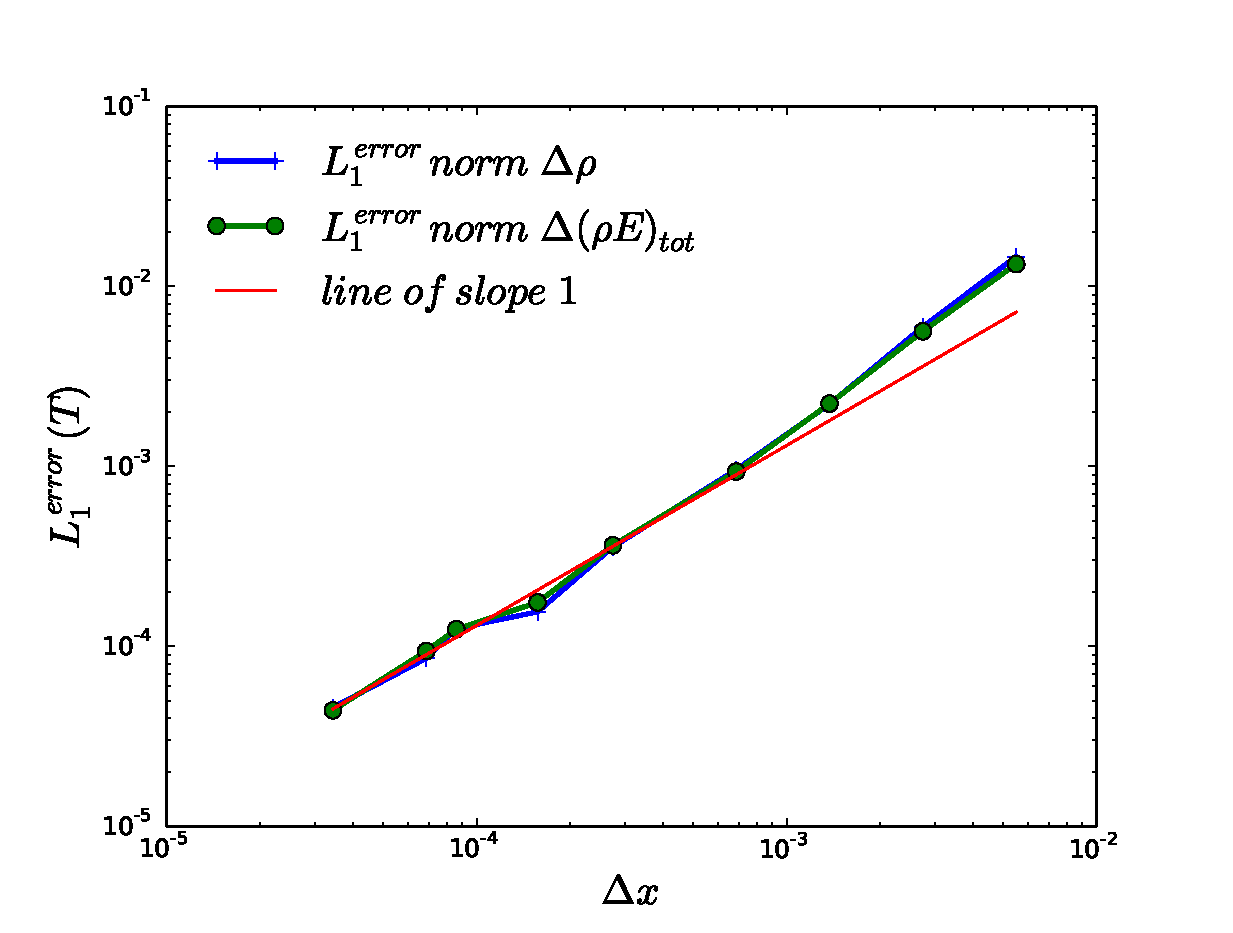
\includegraphics[width=\linewidth]{figures/dpt-xs/mass-energy-diff-scd-method-mat-temp-convergence.eps}
    \caption{Material temperature.}\label{fig:mach-3-dpt-xs-temp-conv}
    \end{subfigure} 
%
    \begin{subfigure}{0.49\textwidth}
    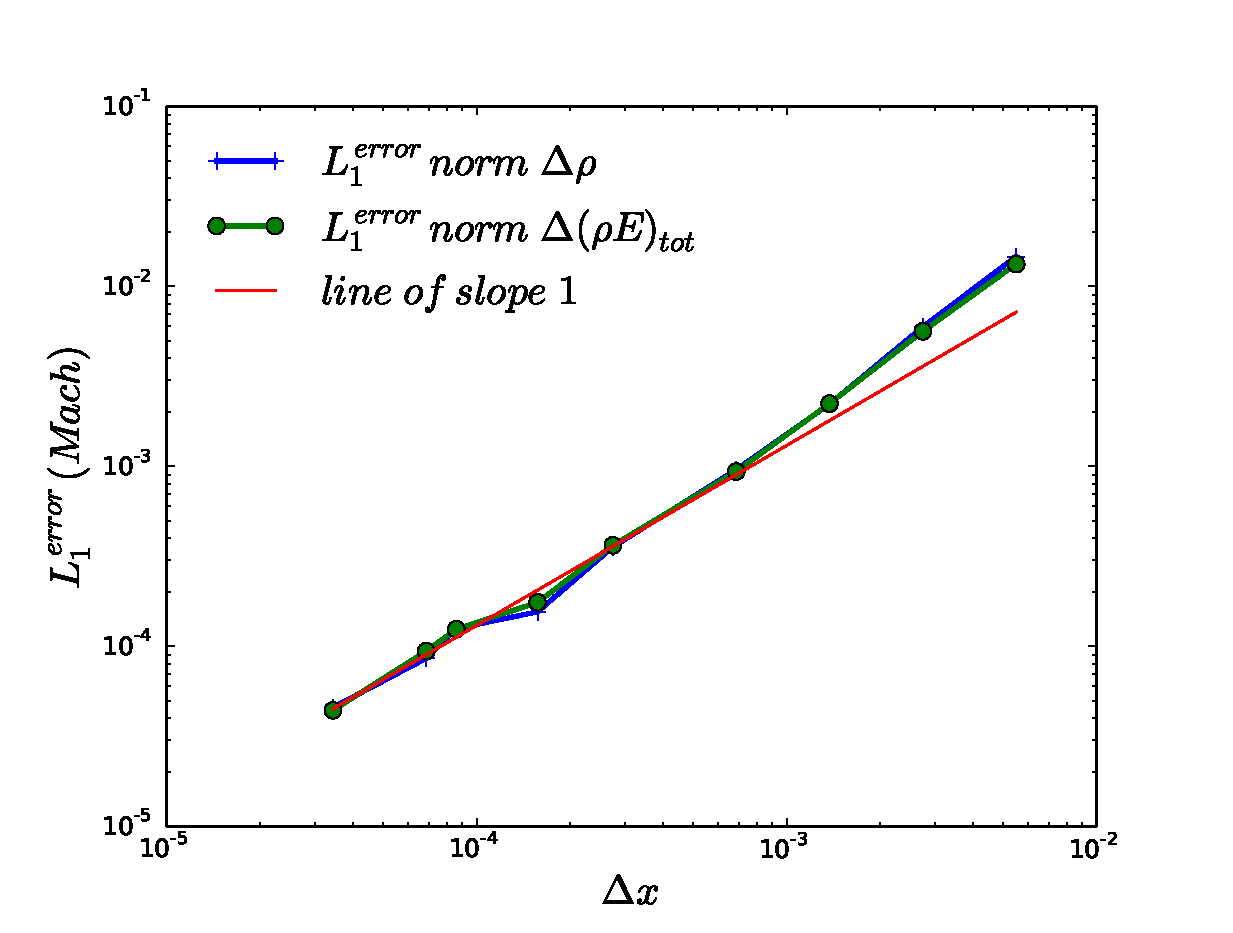
\includegraphics[width=\linewidth]{figures/dpt-xs/mass-energy-diff-scd-method-mach-number-convergence.eps}
    \caption{Mach number.}\label{fig:mach-3-dpt-xs-mach-conv}
    \end{subfigure}
%
    \begin{subfigure}{0.49\textwidth}
    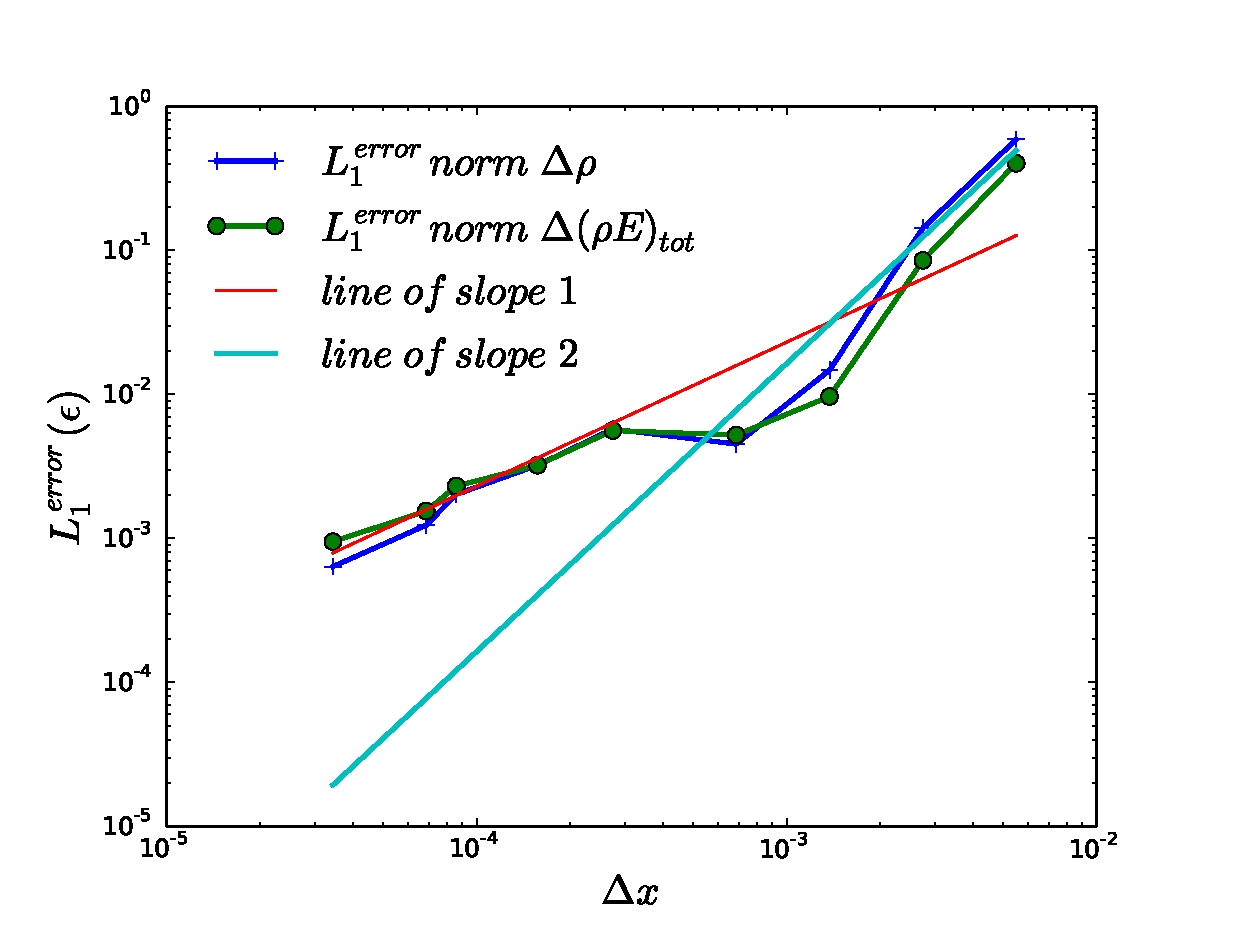
\includegraphics[width=\linewidth]{figures/dpt-xs/mass-energy-diff-scd-method-radiation-convergence.eps}
    \caption{Radiation energy density.}\label{fig:mach-3-dpt-xs-radiation-conv}
    \end{subfigure}        
\caption{Mach $3$ test with density- and temperature-dependent opacity: $L_1$ error norms.}\label{fig:mach-3-dpt-xs-conv} 
\end{figure}
%
\begin{figure}[h]
    \centering
    \begin{subfigure}{0.49\textwidth}
    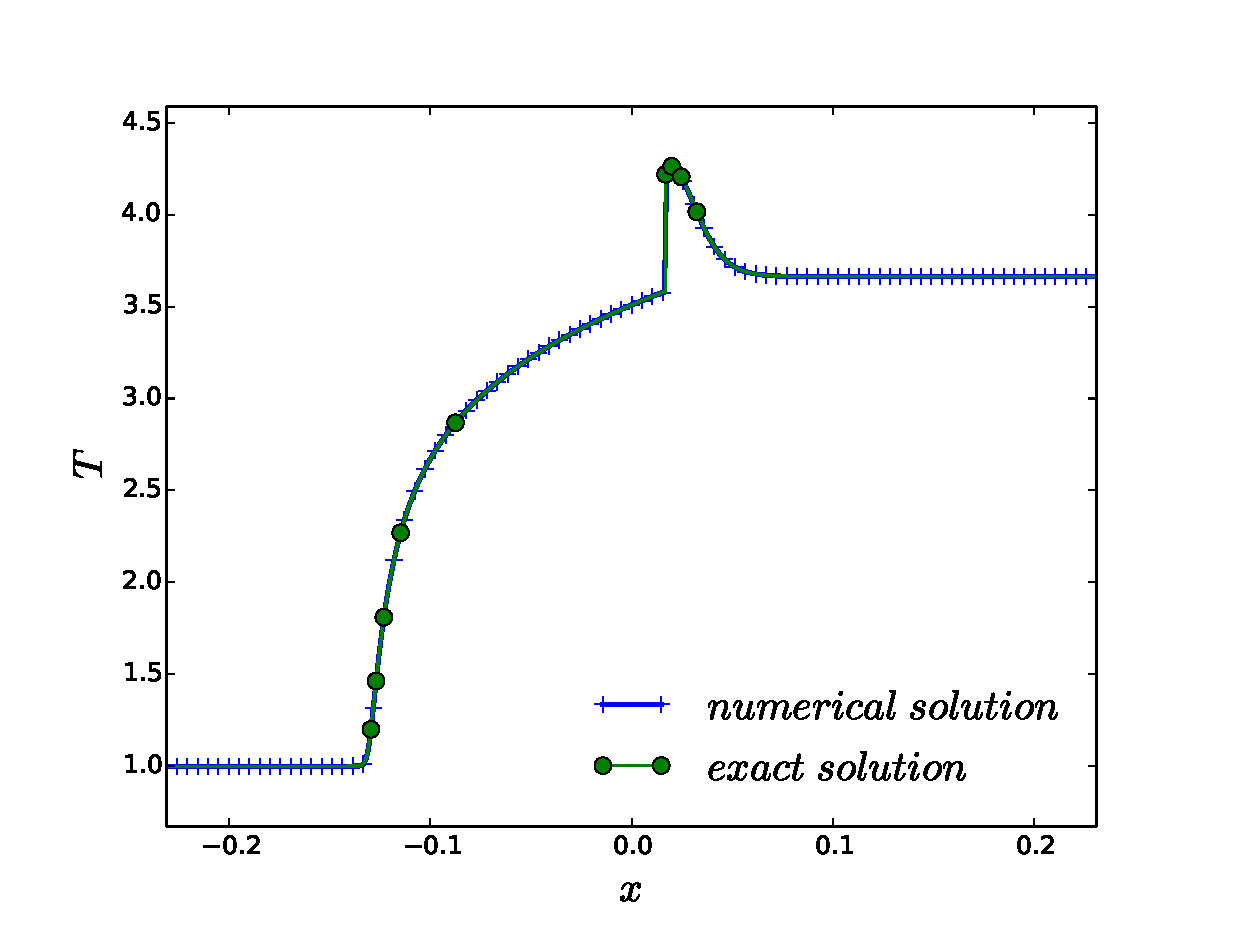
\includegraphics[width=\linewidth]{figures/dpt-xs/mass-diff-mat-temp-nel-2700-plot.eps}
    \caption{Material temperature.}\label{fig:mach-3-dpt-xs-mat-temp}
    \end{subfigure}
%
    \begin{subfigure}{0.49\textwidth}
    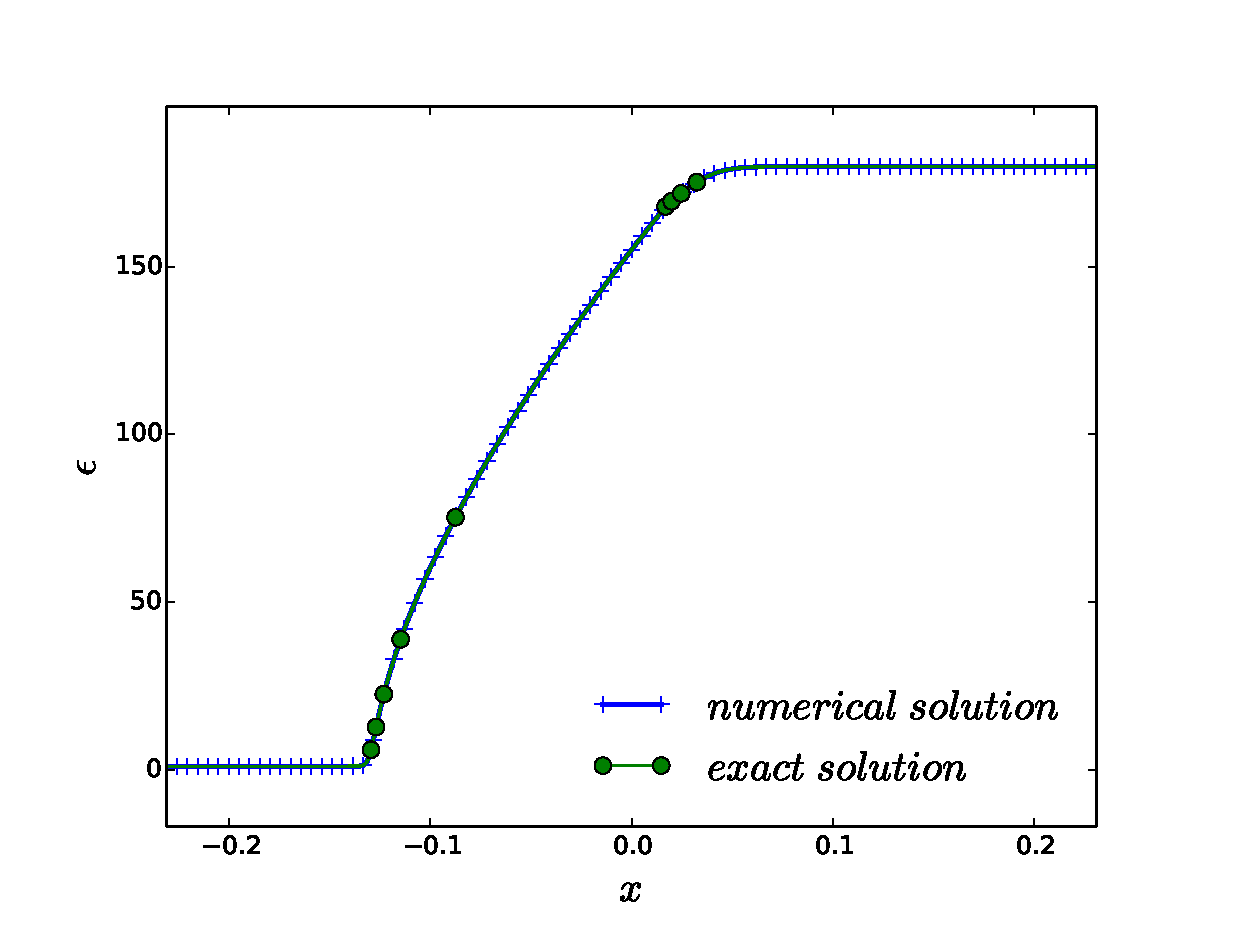
\includegraphics[width=\linewidth]{figures/dpt-xs/mass-diff-radiation-nel-2700-plot.eps}
    \caption{Radiation energy density.}\label{fig:mach-3-dpt-xs-rad-temp}
    \end{subfigure}
%
    \begin{subfigure}{0.49\textwidth}
    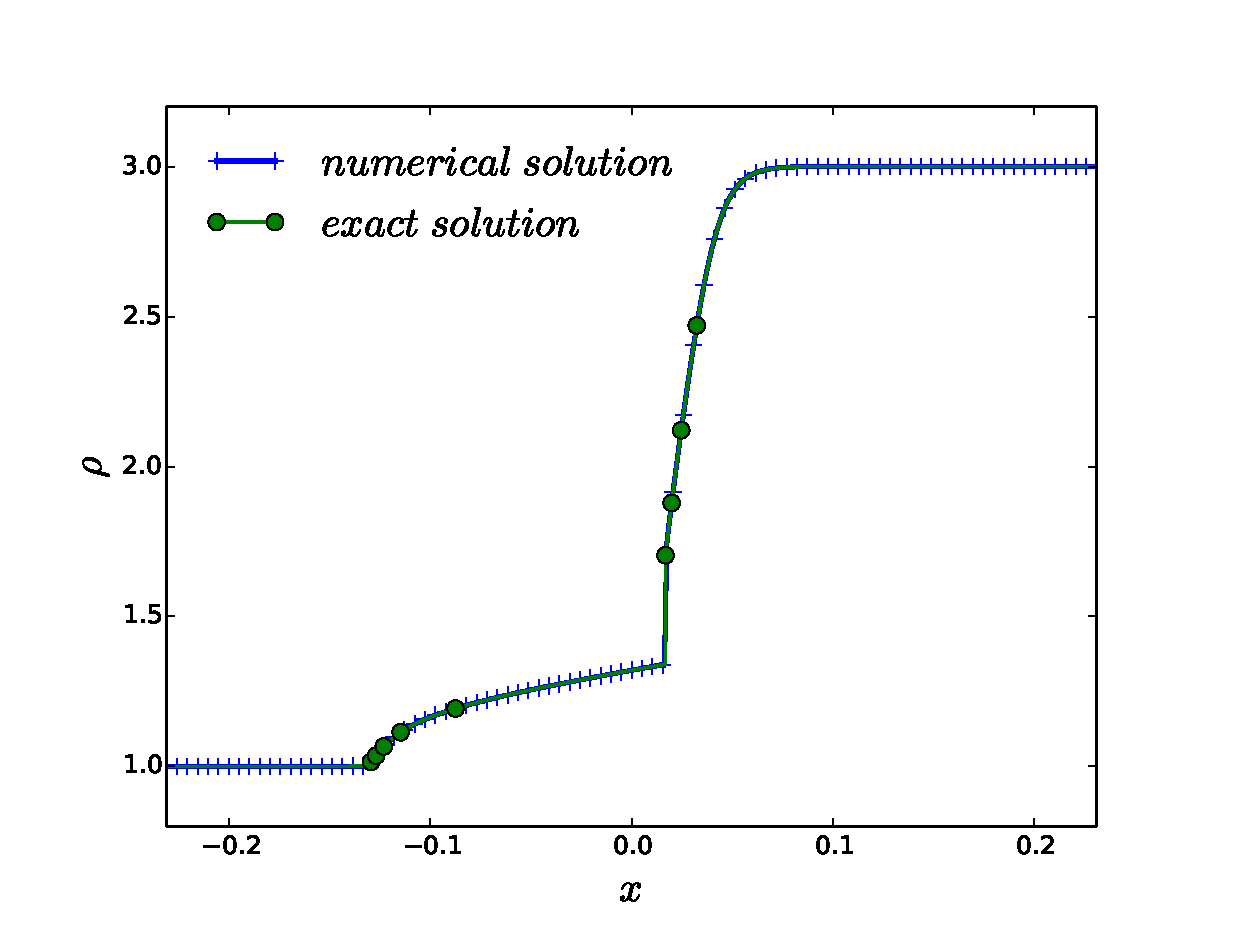
\includegraphics[width=\linewidth]{figures/dpt-xs/mass-diff-density-nel-2700-plot.eps}
    \caption{Material density.}\label{fig:mach-3-dpt-xs-dens}
    \end{subfigure}
%
    \begin{subfigure}{0.49\textwidth}
    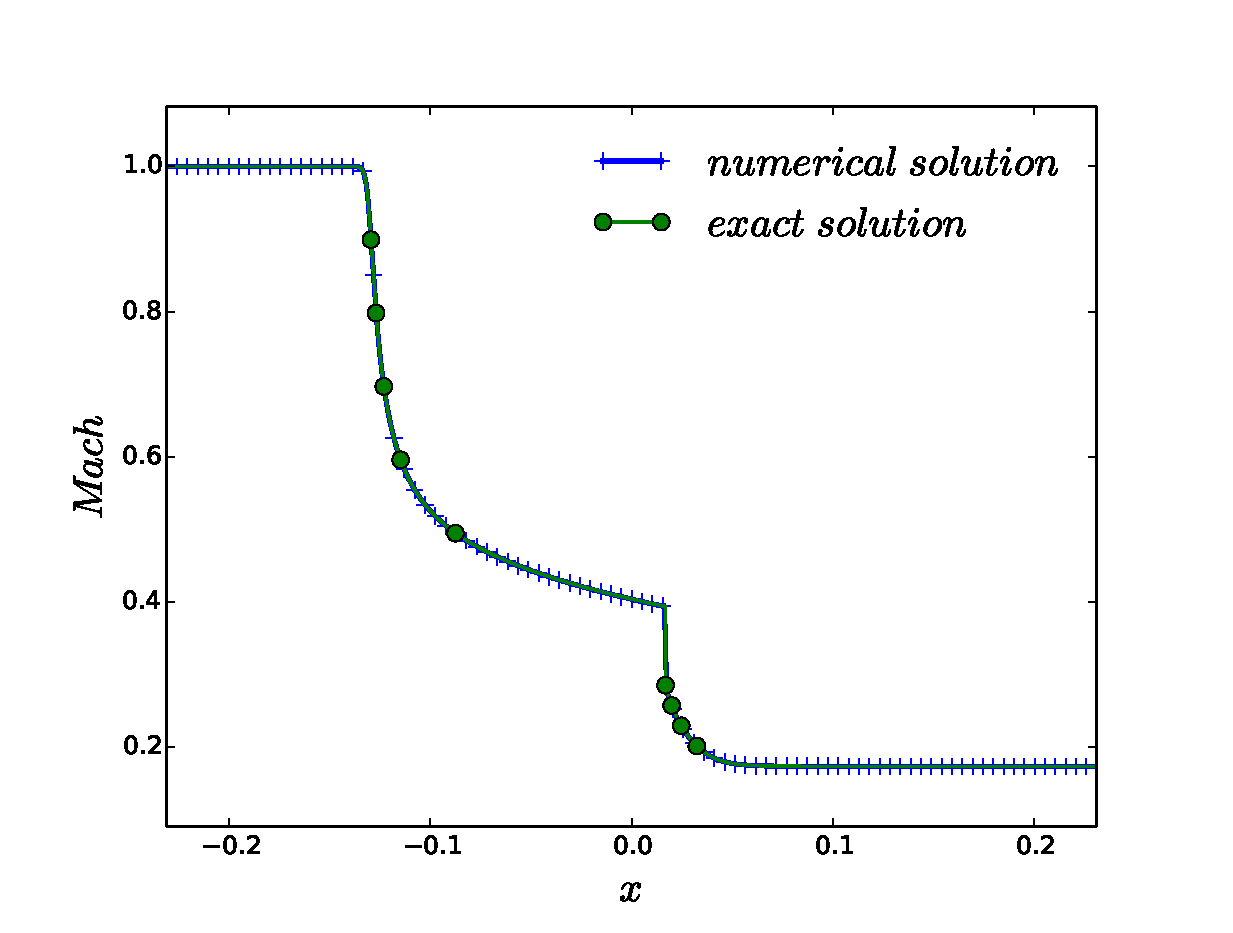
\includegraphics[width=\linewidth]{figures/dpt-xs/mass-diff-mach-number-nel-2700-plot.eps}
    \caption{Mach number.}\label{fig:mach-3-dpt-xs-mach}
    \end{subfigure}
%
    \begin{subfigure}{0.49\textwidth}
    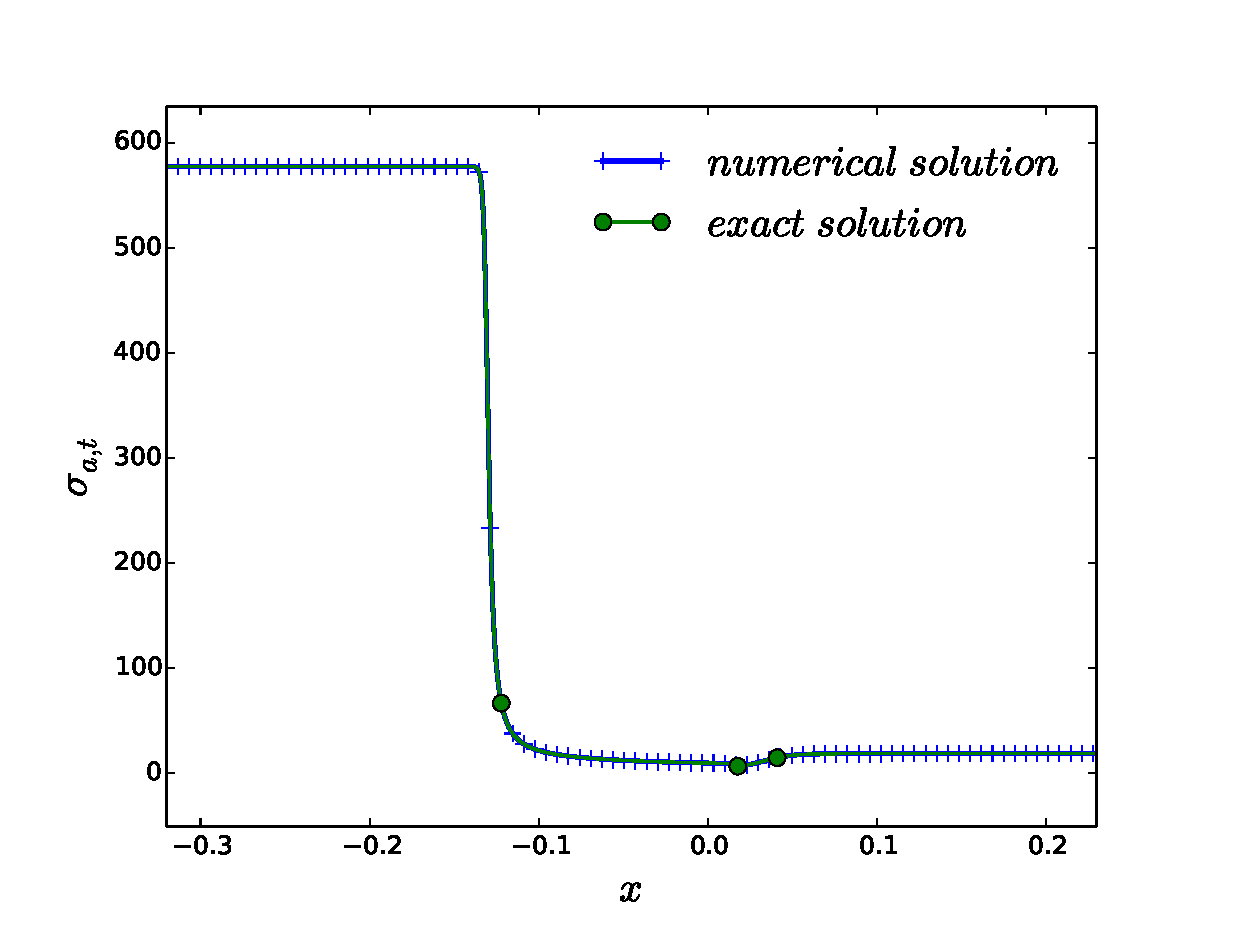
\includegraphics[width=\linewidth]{figures/dpt-xs/mass-diff-opacity-nel-2700-plot.eps}
    \caption{Total opacity $\sigma_t = \sigma_a$.}\label{fig:mach-3-dpt-xs-xs}
    \end{subfigure}
    ~
    \begin{subfigure}{0.49\textwidth}
    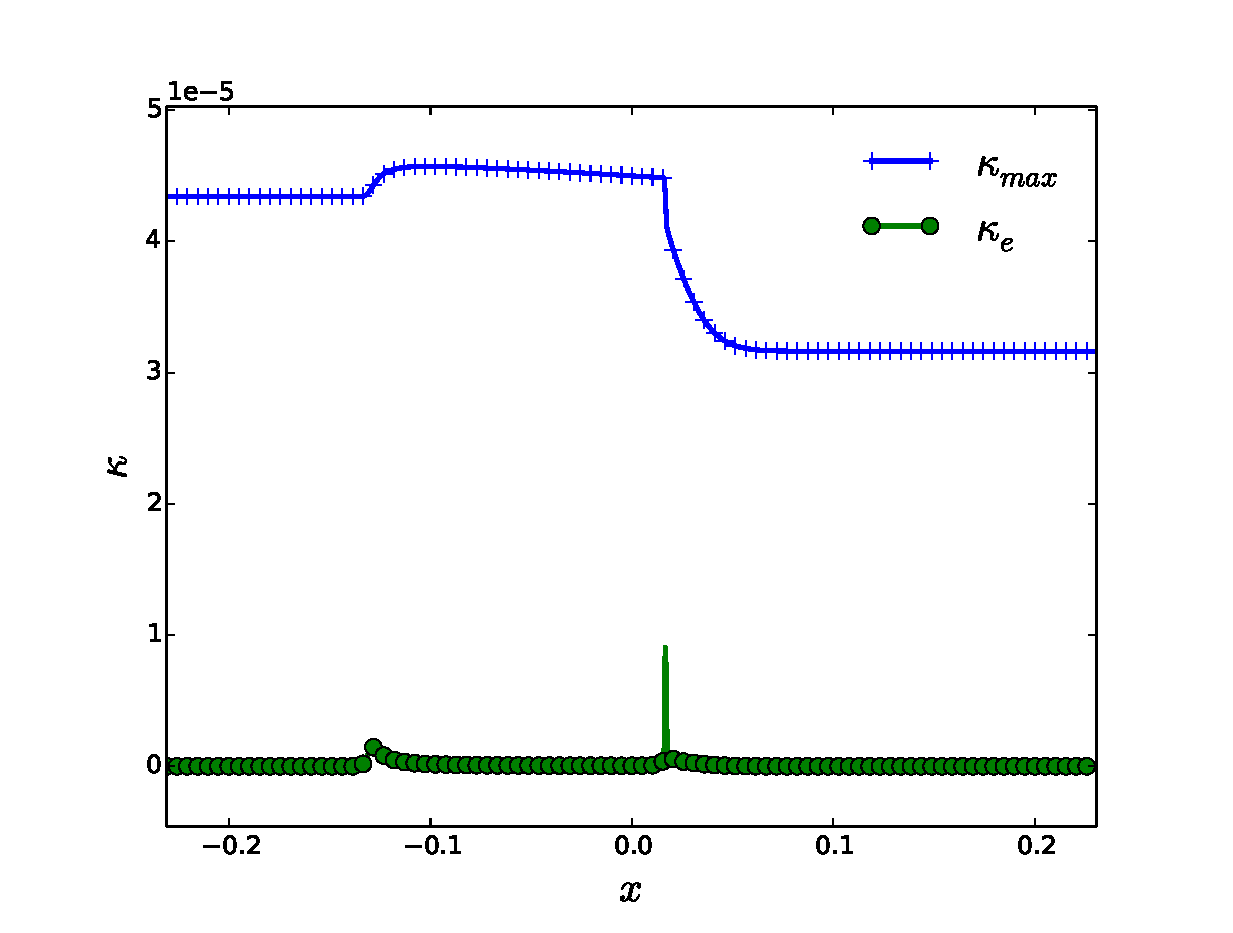
\includegraphics[width=\linewidth]{figures/dpt-xs/mass-diff-visc-nel-2700-plot.eps}
    \caption{Artificial viscosity coefficients.}\label{fig:mach-3-dpt-xs-visc}
    \end{subfigure}      
\caption{Mach $3$ test with density- and temperature-dependent opacity:  Numerical ($2700$ cells) and semi-analytical ($\sim 5 \cdot 10^4$ nodes) steady-state profiles for the material temperature (a), density (b), radiation temperature (c),  Mach number (d), and viscosity coefficient (e).}\label{fig:mach-3-temp-dep-xs}    
\end{figure}
%
The density profile plotted in \fig{fig:mach-3-dpt-xs-dens} does not show any instability neither in the vicinity of the shock around $x \sim 0 \ cm$ nor in the abrupt change located at $x \sim -0.1 \ cm$. The shock is well resolved and the numerical and semi-analytical solutions overlap and are in excellent agreement.
In \fig{fig:mach-3-dpt-xs-mat-temp} and \fig{fig:mach-3-dpt-xs-rad-temp}, the material and radiation temperatures do not show any instability either. The Zeldovich's spike in the material temperature profile is well resolved. The radiation temperature remains smooth as expected because of the diffusion term in the radiation equation. The numerical and semi-analytical solutions are in excellent agreement. 
The profiles of the entropy ($\kappa_e$) and first-order ($\kappa_\text{max}$) viscosity coefficients are shown in \fig{fig:mach-3-dpt-xs-visc}. We observe that the entropy viscosity coefficient $\kappa_e$ displays two peaks at $x\sim-0.1 \ cm$ and at $x \sim 0 \ cm$. The latter one coincides with the shock position where the entropy residual $R_e(x,t)$ is known to peak. % (see \sct{sec:def-visc-coeff} and also \cite{our_jcp_radhy_paper}). 
The former one is due to the inclusion of the jumps in the definition of the entropy viscosity coefficient as recalled in \eqt{eq:visc-def}: the material density does not experience a shock at $x\sim-0.1 \ cm$ but a sharp variation that triggers a larger jump value. 
Once again, even though the entropy viscosity coefficient $\kappa_e$ does not saturate to the first-order viscosity coefficient $\kappa_{max}$, the numerical solution is well behaved thanks to the stabilizing effect of the source terms. %, as explained in \sct{sec:VR_new}.
Overall, the entropy viscosity coefficient behaves as expected: it is peaked in the vicinity of the shock and in regions of sharp variations, and small elsewhere.
%
%------------------------------------------------------------------
%------------------------------------------------------------------
\section{Conclusions and future work}
%------------------------------------------------------------------
%------------------------------------------------------------------
In this paper, the theoretical foundation for the application of the entropy viscosity method to the full nonequilibrium-diffusion Grey Radiation Hydrodynamic equations, i.e., including relaxation and source terms, has been strengthened, utilizing the notions of weak solution and entropy condition for non-conservative hyperbolic systems of equations. We show that 
(i) we still recover an entropy condition that holds for the full set of GRH equations when borrowing the functional expression of the entropy  $s(\rho,e,\varepsilon)$ previously derived by only considering the hyperbolic parts of the GRH \cite{our_jcp_radhy_paper}, and
(ii) the same viscous regularization can be employed to stabilize the GRH equations.
Using the above theoretical results, the definition of the first-order and entropy-viscosity coefficients from \cite{our_jcp_radhy_paper} are shown to be still valid. 

The EVM was tested with various test cases and the numerical solutions were compared against semi-analytical solutions obtained by following the method described in \cite{LowrieEdwards}. We proposed mass and energy conservation procedures to align numerical and semi-analytical solutions. Convergence studies show that second-order accuracy is obtained for smooth solutions (Mach 1.05 test case) and that solutions with shocks (Mach 3 test cases) yield first-order accuracy in all variables for fine meshes. For the Mach 3 test cases, we also observed that the radiation energy density achieves second-order accuracy on coarse meshes (pre-asymptotic region).

Physical features such as embedded hydrodynamic shocks and the Zeldovich spike are resolved accurately without spurious oscillations. The entropy viscosity coefficient is only peaked in the vicinity of the shock and in region of strong gradients, and remains small elsewhere, as expected. Overall, the entropy viscosity method behaves very satisfactorily when compared against semi-analytical solutions.

%
Future work will include extension to multi-dimensional simulations and the use of an $S_n$ radiation transport approximation to model the radiation energy density distribution.

%%%%%%%%%%%%%%%%%%%%%%%%%%%%%%%%%%%%%%%%%%%%%%%%%%%%%%%%%%%%%
%%%%%%%%%%%%%%%%%%%%%%%%%%%%%%%%%%%%%%%%%%%%%%%%%%%%%%%%%%%%%
\section*{Acknowledgments}
The authors would like to acknowledge Robert Lowrie (LANL), Bojan Popov (TAMU), and Jim Morel (TAMU) for many fruitful discussions.
%%%%%%%%%%%%%%%%%%%%%%%%%%%%%%%%%%%%%%%%%%%%%%%%%%%%%%%%%%%%%
%%%%%%%%%%%%%%%%%%%%%%%%%%%%%%%%%%%%%%%%%%%%%%%%%%%%%%%%%%%%%

\appendix

\section{Implementation of boundary conditions} \label{App:AppendixA}

This appendix deals with the implementation of the boundary conditions for the Grey Radiation-Hydrodynamic equations solved with a \emph{continuous Galerkin finite element method} and with an \emph{implicit temporal solver}. The boundary condition terms arise from the following conservative terms:
%
\begin{equation}\label{eq:bc-fluxes}
F(U) + D(U) = 
\begin{bmatrix}
\rho u \\
\rho u^2 + P + \frac{\epsilon}{3} \\
u \left( \rho E + P \right) \\
\frac{4}{3} u \epsilon
\end{bmatrix}
+  
\begin{bmatrix}
0 \\
0 \\
0 \\
- \frac{c}{3 \sigma_t} \partial_x \epsilon
\end{bmatrix}
\,.
\end{equation}
%
To discretize the conservative fluxes F(U) and D(U) in a finite element approach, one multiplies by a test function $\phi$, and integrates by parts over the computational domain. The resulting boundary terms are as follows:
%
\begin{eqnarray}
\left[\left(F(U)+D(U)\right) \cdot \vec{n} \ \phi \right]_{l} - \left[ \left(F(U)+D(U)\right) \cdot \vec{n} \ \phi \right]_{r} \, ,
\end{eqnarray}
%
where $\vec{n}$ is the outward normal at the left $l$ and right $r$ boundaries. 
In the following sections, we first give the implementation of the boundary conditions for the first-order differential terms, i.e., the advection terms, and then deal with the second-order differential term found in the radiation-diffusion equation. 
%
\subsection{Implementation of the boundary terms for $F(U)$}
%
Study of the hyperbolic term of the 1-D GRH equations yield four eigenvalues that are $\lambda_{1,2}=u$ and $\lambda_{3,4}=u \pm c_m$. The sign of the eigenvalues inform us on how the physical information travel in the computational domain and at the boundaries. We consider in the appendix the cases of a left supersonic and a right subsonic boundaries as they are of interest to the tests presented in this paper. Under the assumption of a supersonic left boundary condition ($u \geq c_m$), all eigenvalues are positive and no physical information leaves the computational domain. As a result, four boundary values, ($\rho_{l, user}, u_{l, user}, P_{l, user}, \epsilon_{l, user})$, must be user-specified and, along with an equation of state, are used to compute the boundary flux $F(U)$. 

In the other hand, the treatment of the right subsonic boundary, ($u \leq c_m$), is quite different as three eigenvalues are positive and one is negative, meaning, physical information leaves and enters the computational domain at the right boundary. Consequently, the right boundary fluxes from the advection terms are computed using one user-specified boundary value, typically the material pressure $P_{r, user}$, and three boundary values supplied by the code, i.e., current values of the material density ($\rho_{r}$) velocity ($u_{r}$) and radiation energy density ($\epsilon_{r}$). Using an equation of state along with the user-specified and current boundary values, the boundary flux $F(U)$ is computed.
%
\subsection{Implementation of the boundary terms for $D(U)$}
%
The radiation-diffusion equation contains the elliptic term $D(U)$ that yields the boundary term 
%
\begin{eqnarray}
\left[D(U)\cdot \vec{n} \ \phi \right]_{l} - \left[D(U)\cdot \vec{n} \ \phi \right]_{r} \, . \nonumber
\end{eqnarray}
%
A reflective boundary condition, i.e. $\left. \partial_x \epsilon \right|_j = 0$, is used to implement the boundary flux from the diffusion term
which implies $\left[D(U)\cdot \vec{n} \ \phi \right]_{j} = 0$ for $j = \left( l, \ r \right)$.

%%%%%%%%%%%%%%%%%%%%%%%%%%%%%%%%%%%%%%%%%%%%%%%%%%%%%%%%%%%%%
%%%%%%%%%%%%%%%%%%%%%%%%%%%%%%%%%%%%%%%%%%%%%%%%%%%%%%%%%%%%%

\bibliography{mybibfile}
\end{document}
